\chapter{Design}

\section{Overall System Design}

\subsection{Short description of the main parts of the system}

\begin{itemize}
	\item Restaurant Simulator
	\begin{itemize}
		\item Core Elements of System
		\item General User Interface
		\item Adding Item
		\item Deleting Item
		\item Saving Order Information
		\item Managing Bookings
		\item Managing Item Menu

	\end{itemize}
		
\end{itemize}

Core Elements of System
\\
The system will be designed to make it easier to track information about the restaurant for the restaurant staff, information will be displayed on the application. Information tracked down includes order information such as what has been ordered by each table and the information about that table like the number of people, date  and time arrived. In addition, booking times will be displayed at the main screen. As well as displaying key information, the system will have features to add/delete/edit information. For example, adding items to an order, deleting irrelevent bookings and editing booking times. The core elements of the system will be based on managing orders and bookings.

General User Interface
\begin{itemize}
	\item Only staff will be able to access this application, so a box will be the first thing that prompts up when the applicaiton is opened. This box will require staff members to enter a password which they have created.
	\item After entering the correct password, the application will display the layout of restaurant in a birds eye view way. The layout will contain shapes which represent each table, each shape will have the number of table on it.
	\item Clicking on table will bring up a box with a layout like an invoice such as the one on page 15.This screen will contain the table's status such as what they ordered, date,time, table number, number of people and total price. The main box in the middle will be split in half where the left half will contain the dishes ordered and the right will contain the drinks ordered. At the bottom will be contain the editing features where there will be an Add, Delete and Finish buttons. In addition, there will be a back arrow at the top and once  this is clicked, it will return to the main interface with the restaurant layout and save the order information.

\end{itemize}

Adding Item
\begin{itemize}
	\item The managing order box that pops up when clicked on a table, will have an 'Add' button at the bottom. This button will have the feature to add a menu item to the order.
	\item When the 'Add' button is clicked, a box will pop up where the user enters the name or item ID and if name or ID is entered correctly, the item will appear on the table status. The menu will be displayed to aid the user.
\end{itemize}

Deleting Item
\begin{itemize}
	\item The managing order box will have a 'Delete' button located at the bottom. This button will have the feature to delete a menu item off the order
	\item When the 'Delete' button is clicked, red boxes with an X will appear next to each item ordered. If the red button is clicked, the item will disappear off the order.
\end{itemize}

Saving Order Information
\begin{itemize}
	\item A 'Finish' button will be located along with the 'Add' and 'Delete' buttons. 
	\item The 'Finish' button will be used once a table has finished eating/ordering. It will save all of the current information about this particular order. 
	\item Information will be the ordered menu items, table number, date, time, number of people and the total price.
\end{itemize}

Managing Bookings
\begin{itemize}
	\item Any table bookings will be displayed on the main screen 
	\item A button labelled "Bookings" will be at the main screen. A box will appear that will be used to manage bookings.
	\item Adding and deleting bookings will be available through this box that is used to manage bookings.
\end{itemize}

Managing Item Menu
\begin{itemize}
	\item There will be an option to add an item to the menu or delete an item off the menu. This will be accessed at the menu bar.
	\item The menu bar will have a drop down box containing "Add Item" "Delete Item"
	\item Adding an item requres the user to input the information required.
	\item Deleting an item will be done by the user entering either the name of the item or the ID. The menu will be displayed to aid the user.
\end{itemize}

\subsection{System flowcharts showing an overview of the complete system}

\begin{figure}[H]
    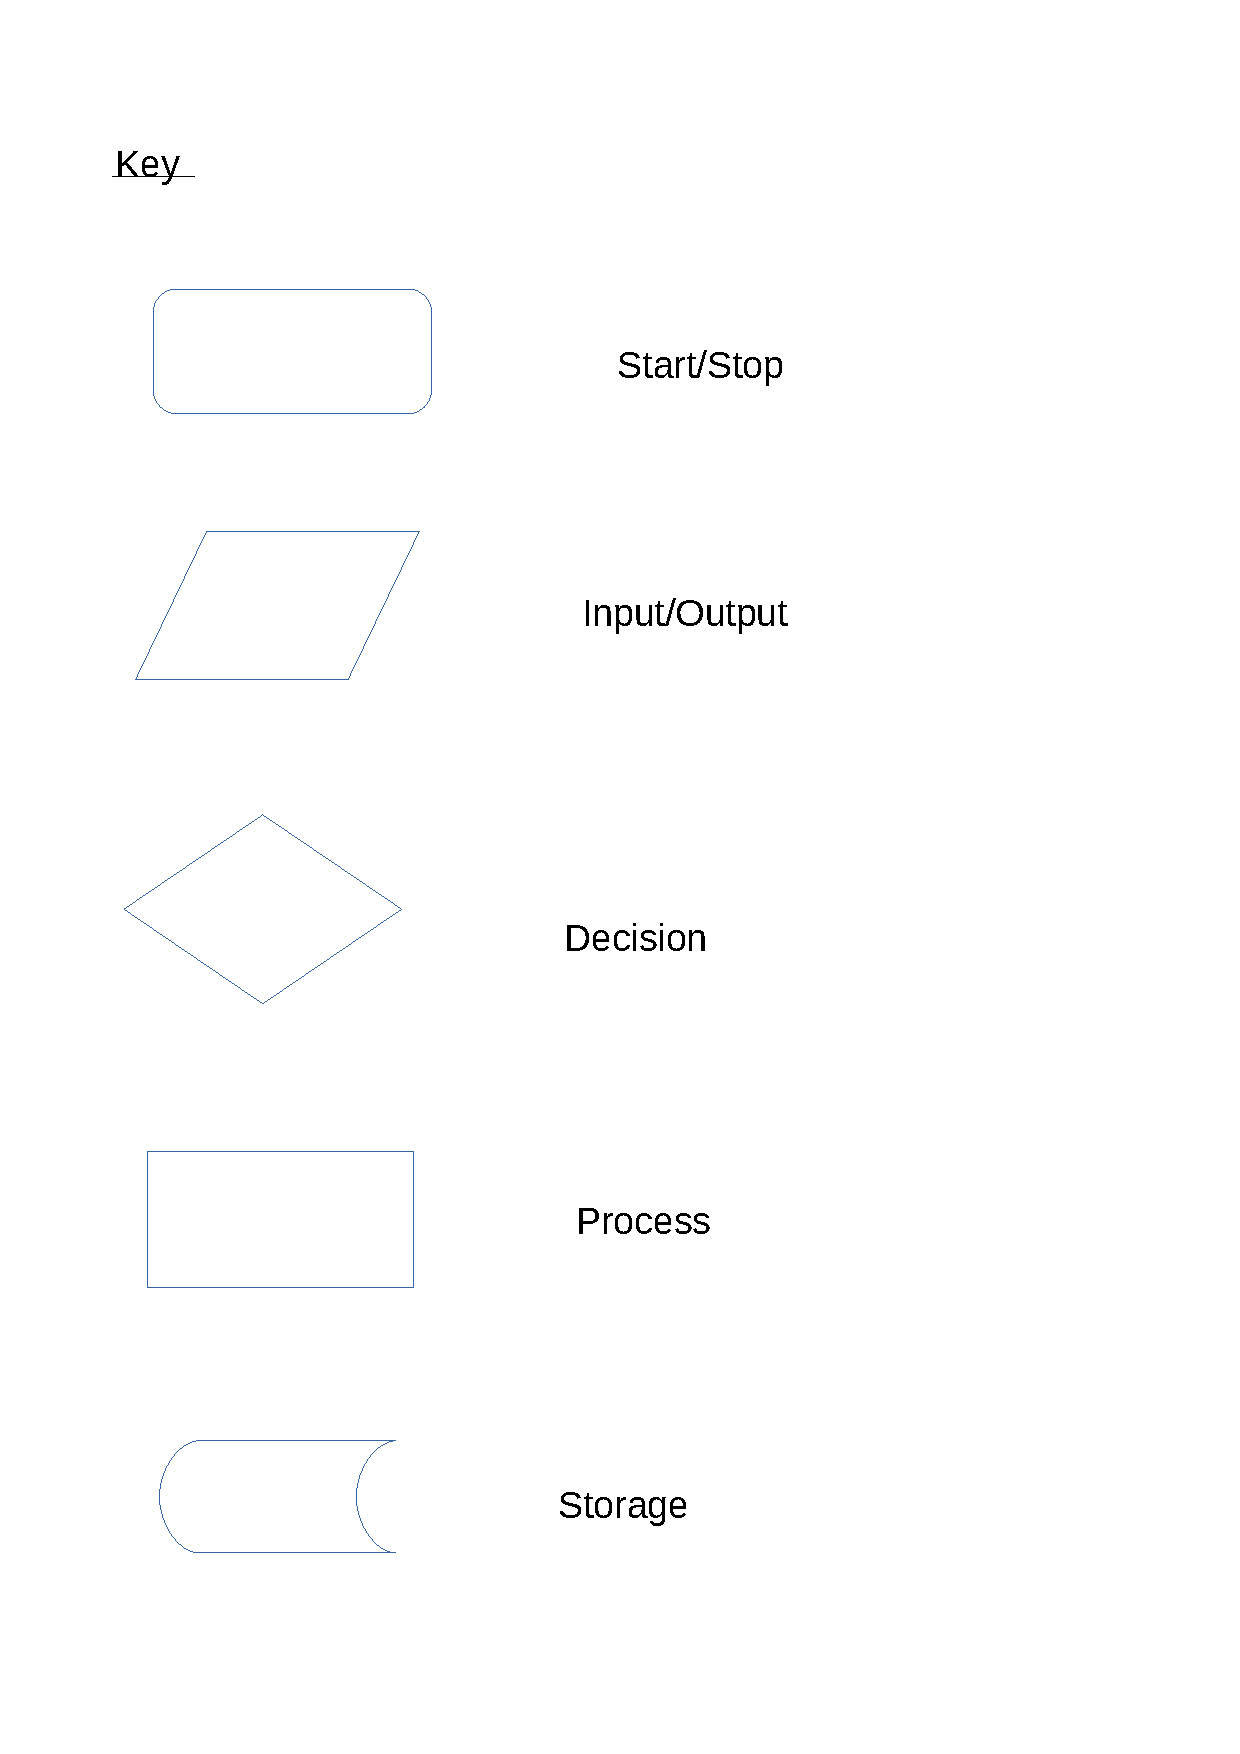
\includegraphics[height = 20cm]{./Design/Images/flowchart0}
    \caption{Key for flowchart} \label{fig:Flowchart0}
\end{figure}

\begin{figure}[H]
    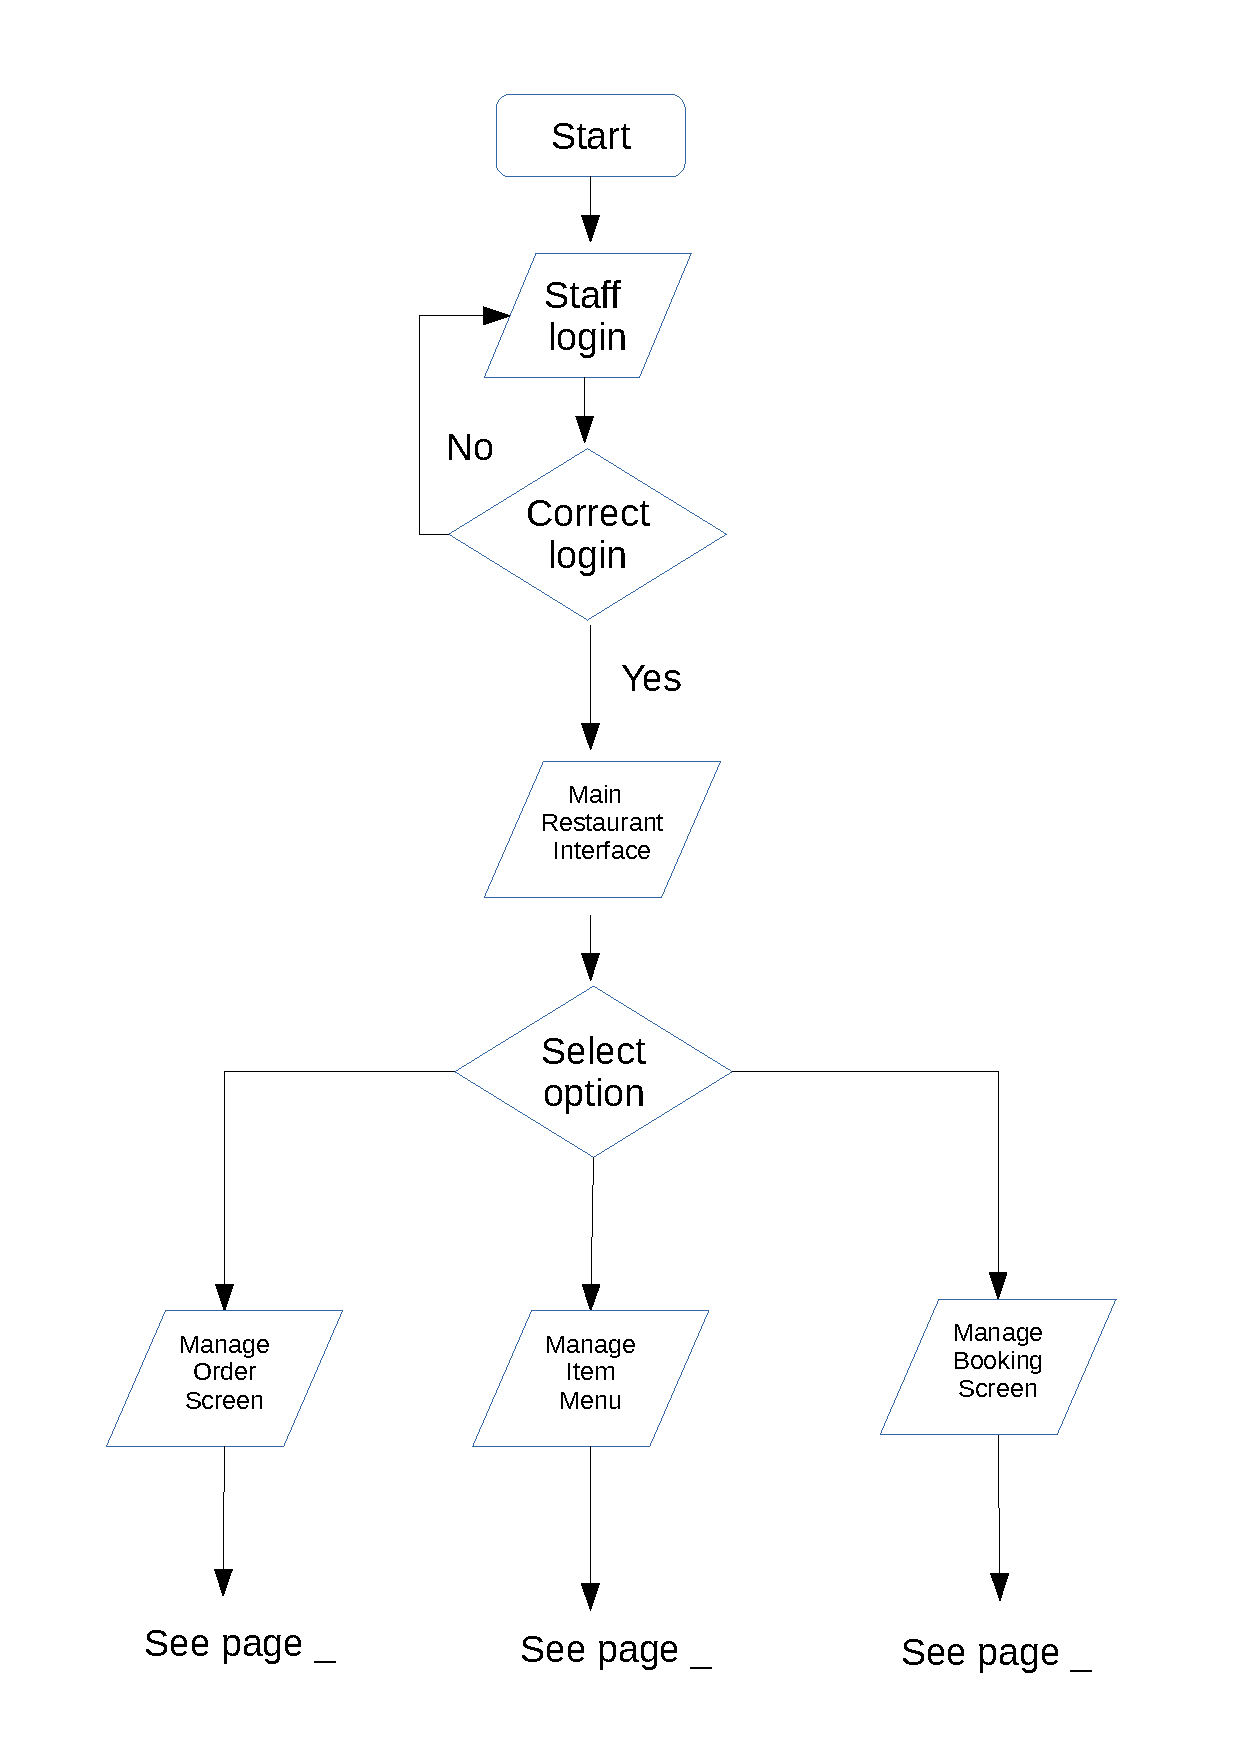
\includegraphics[height = 20cm]{./Design/Images/flowchart1}
    \caption{Flow chart of system} \label{fig:Flowchart1}
\end{figure}

\begin{figure}[H]
    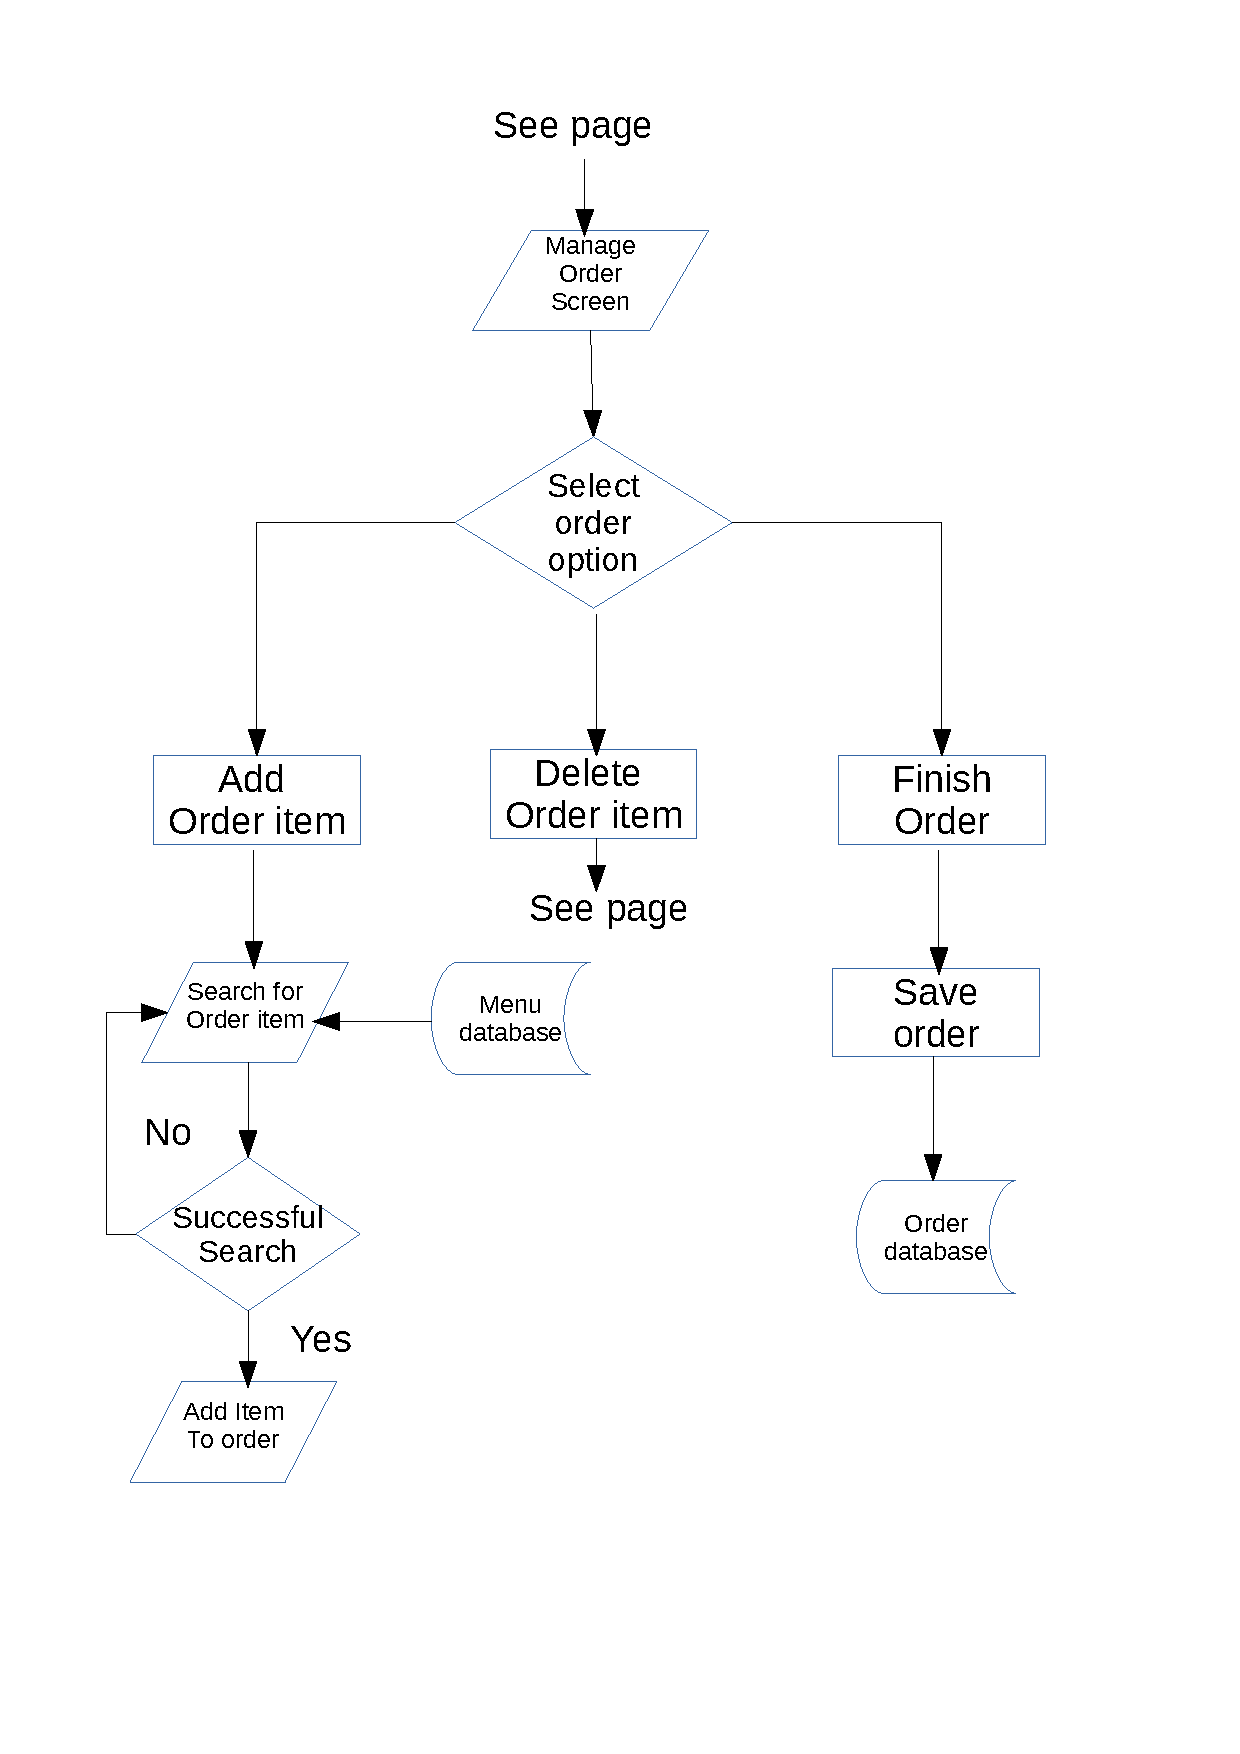
\includegraphics[height = 20cm]{./Design/Images/flowchart2}
    \caption{Flow chart of order} \label{fig:Flowchart2}
\end{figure}

\begin{figure}[H]
    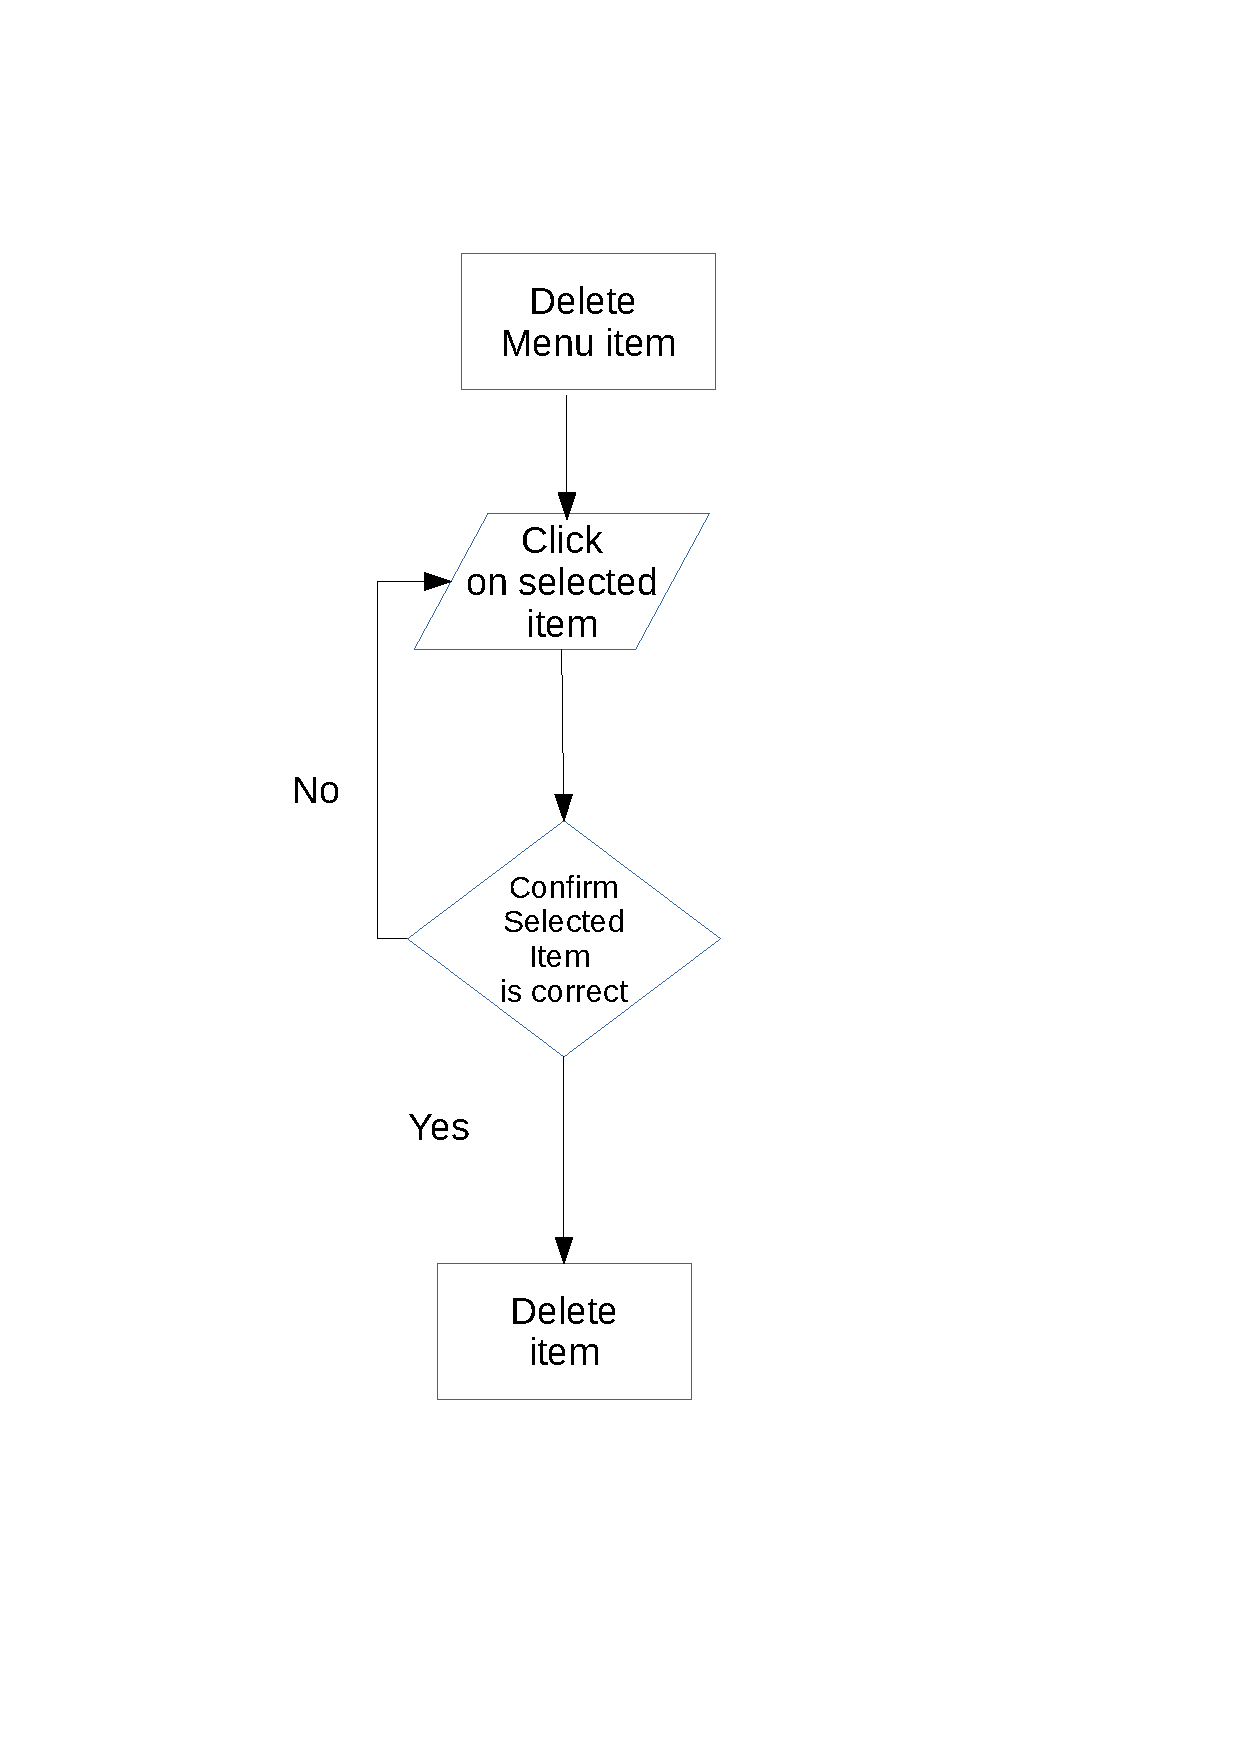
\includegraphics[height = 20cm]{./Design/Images/flowchart3}
    \caption{Flow chart of deleting an item of an order} \label{fig:Flowchart3}
\end{figure}

\begin{figure}[H]
    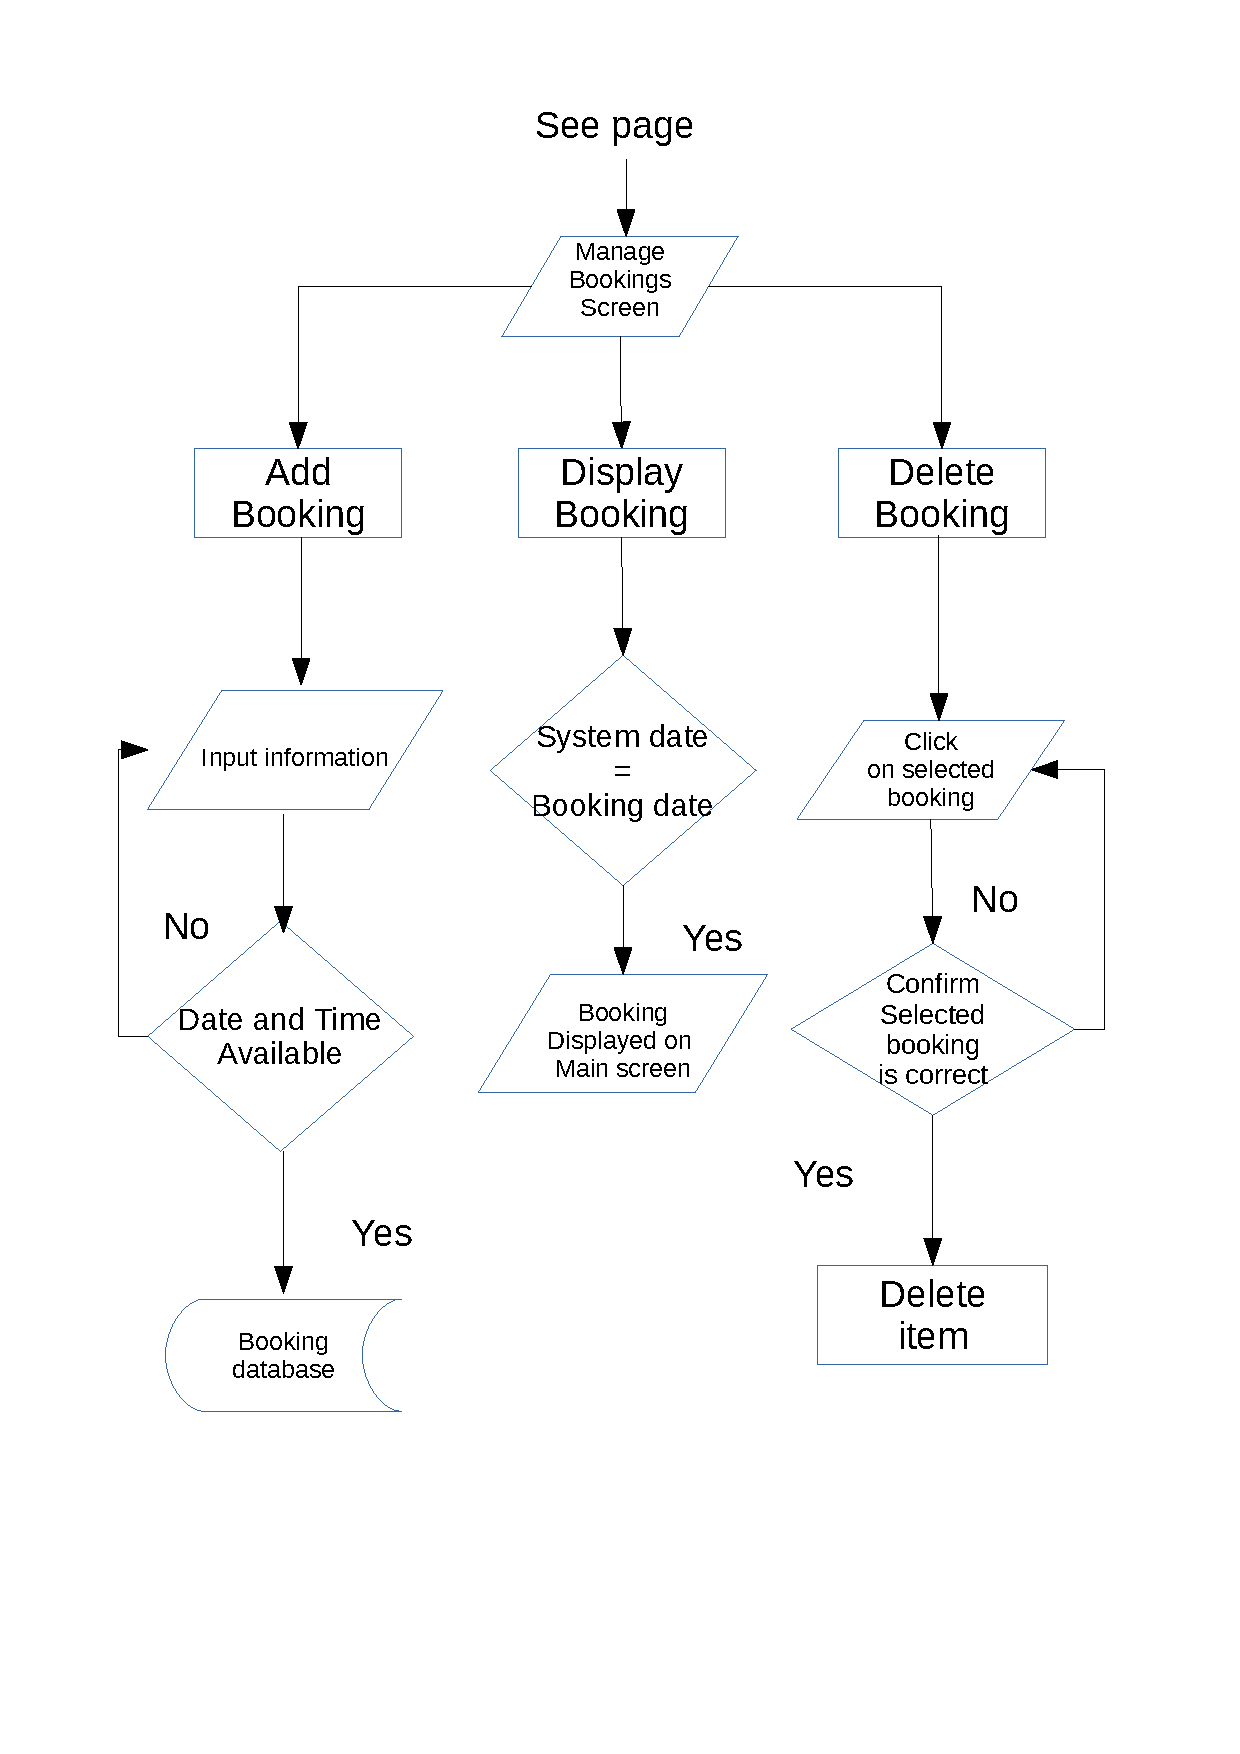
\includegraphics[height = 20cm]{./Design/Images/flowchart4}
    \caption{Flow chart of bookings} \label{fig:Flowchart4}
\end{figure}

\begin{figure}[H]
    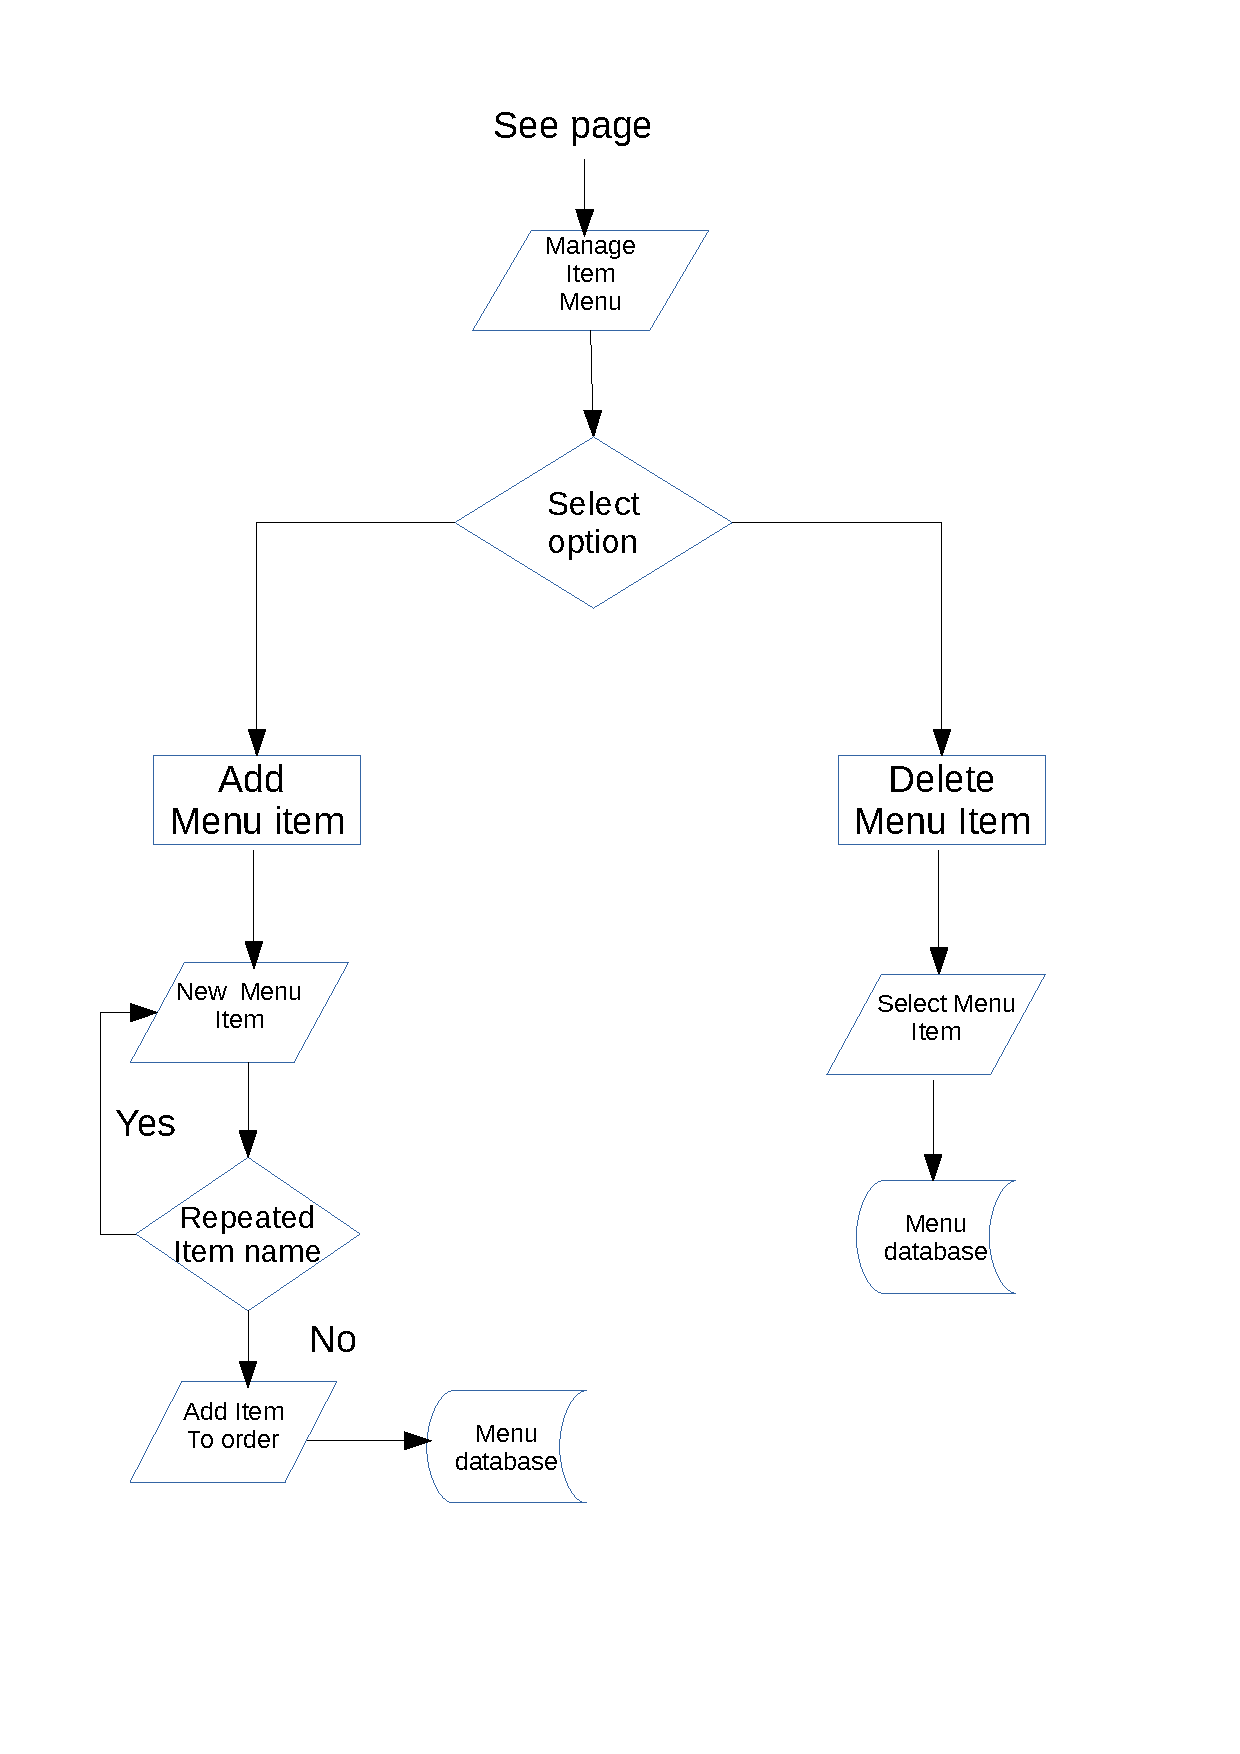
\includegraphics[height = 20cm]{./Design/Images/flowchart5}
    \caption{Flow chart of adding an item to the menu} \label{fig:Flowchart5}
\end{figure}


\section{User Interface Designs}

\begin{figure}[H]
    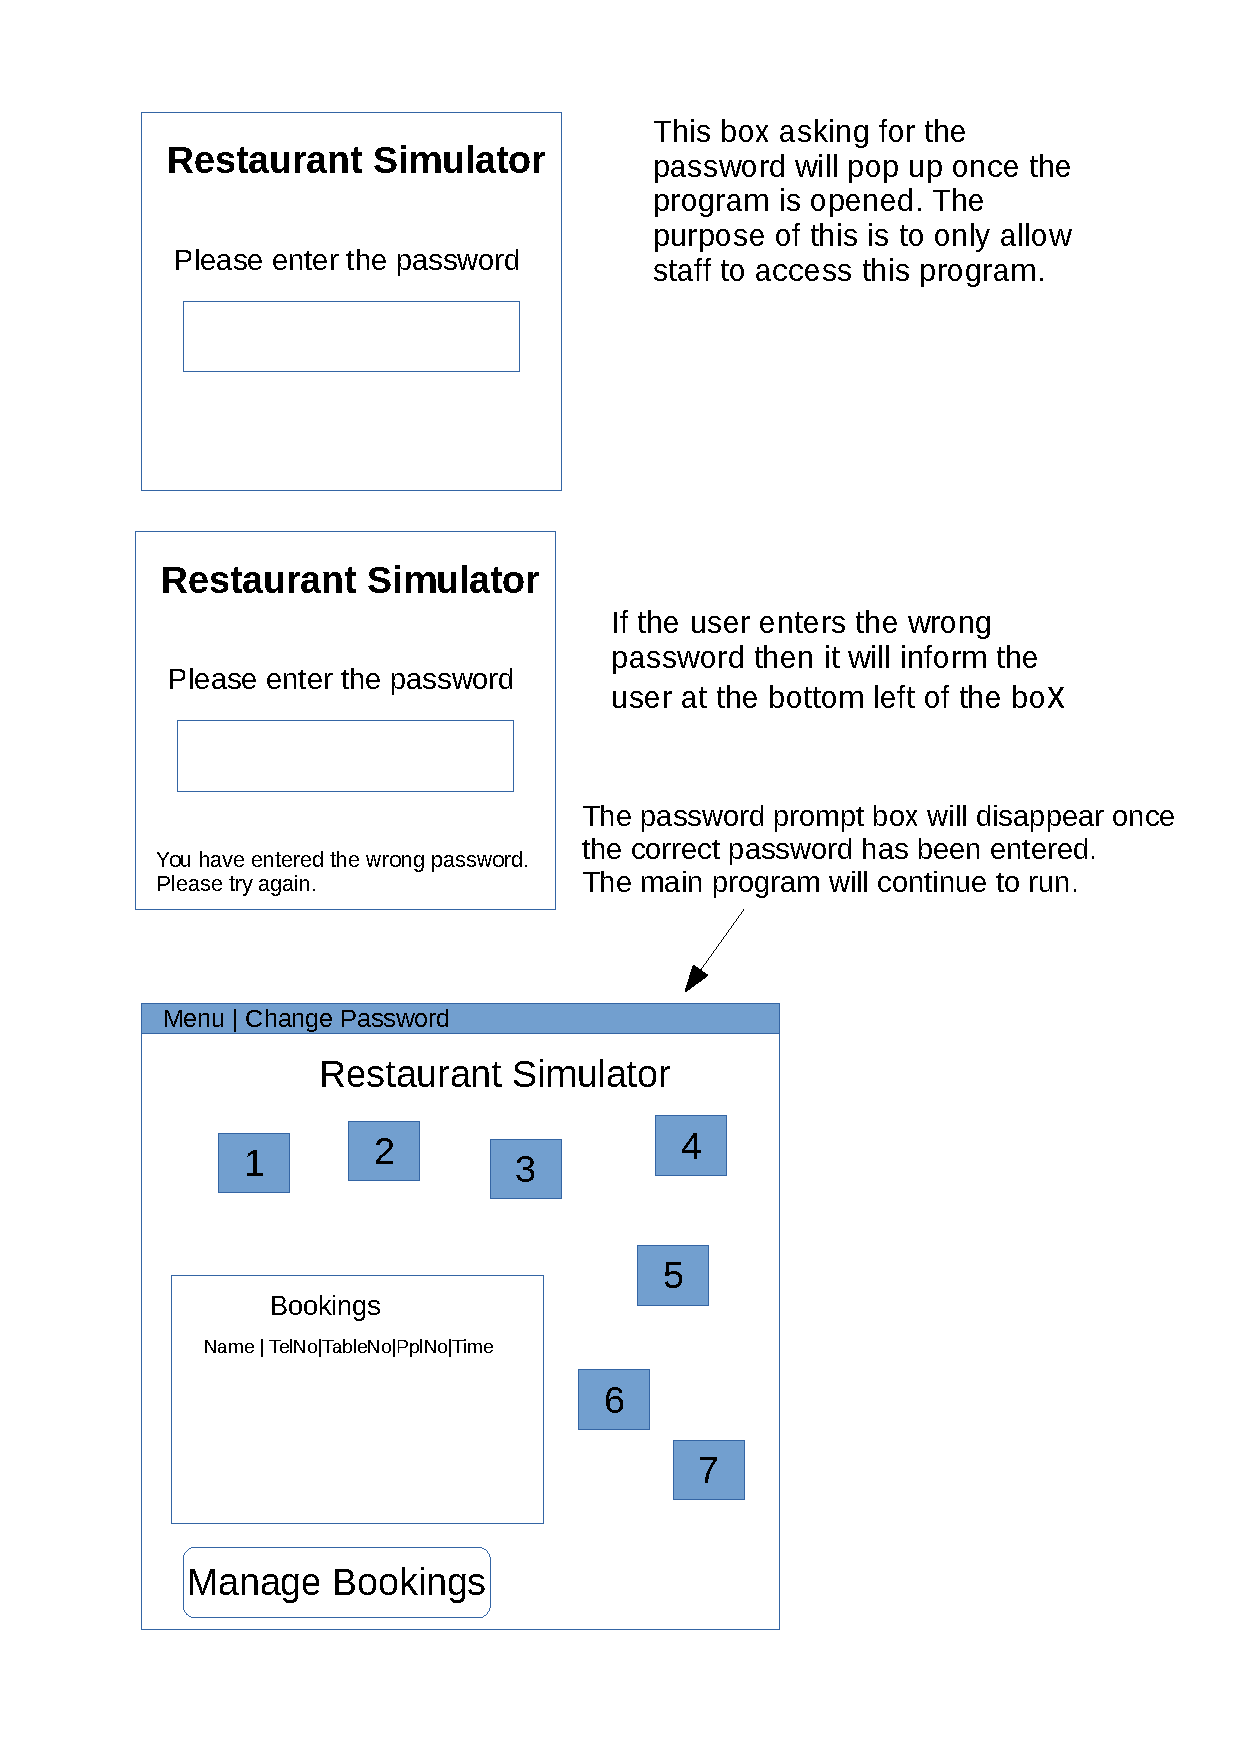
\includegraphics[height = 20cm]{./Design/Images/Interface1}
    \caption{Password Prompt} \label{fig:Password}
\end{figure}

\begin{figure}[H]
    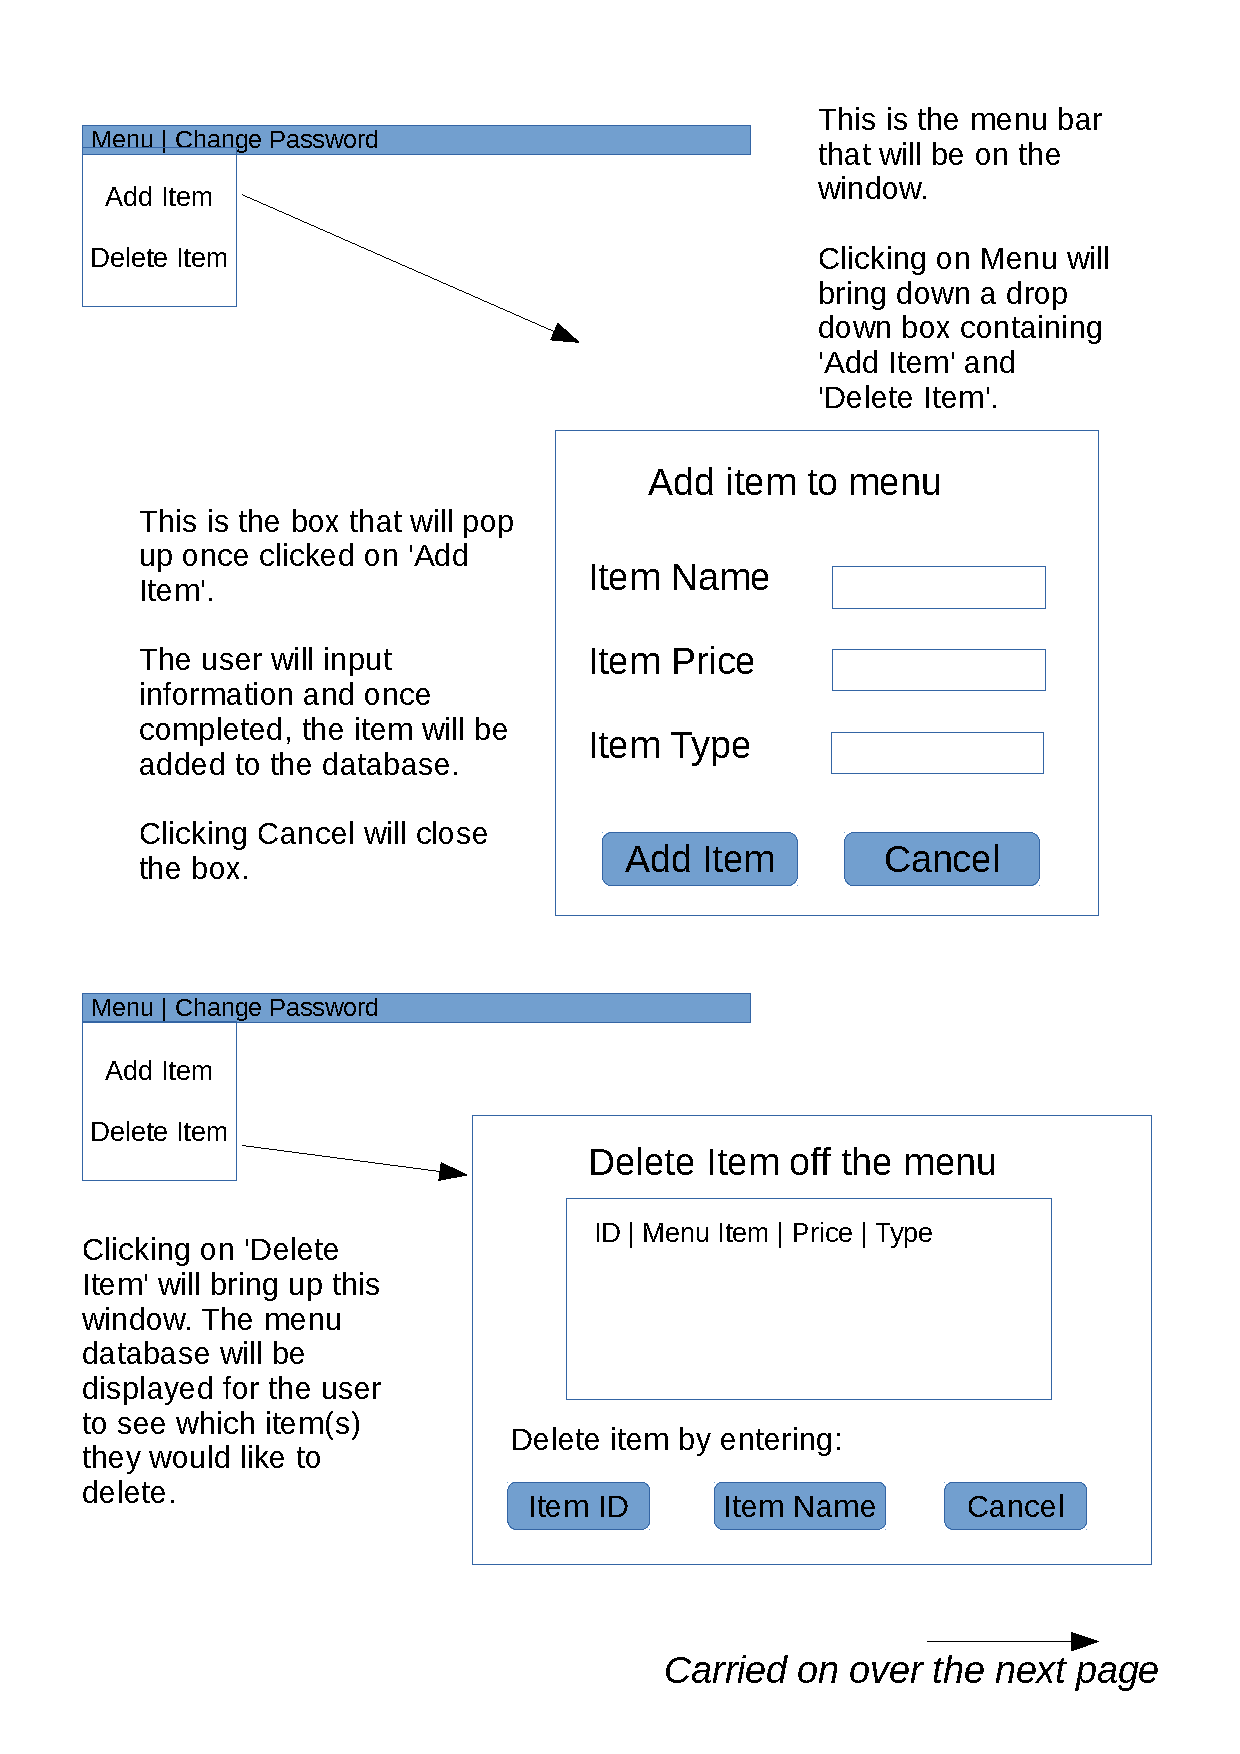
\includegraphics[height = 20cm]{./Design/Images/InterfaceMenuBar}
    \caption{Explaining Menu Bar} \label{fig:MenuBar}
\end{figure}

\begin{figure}[H]
    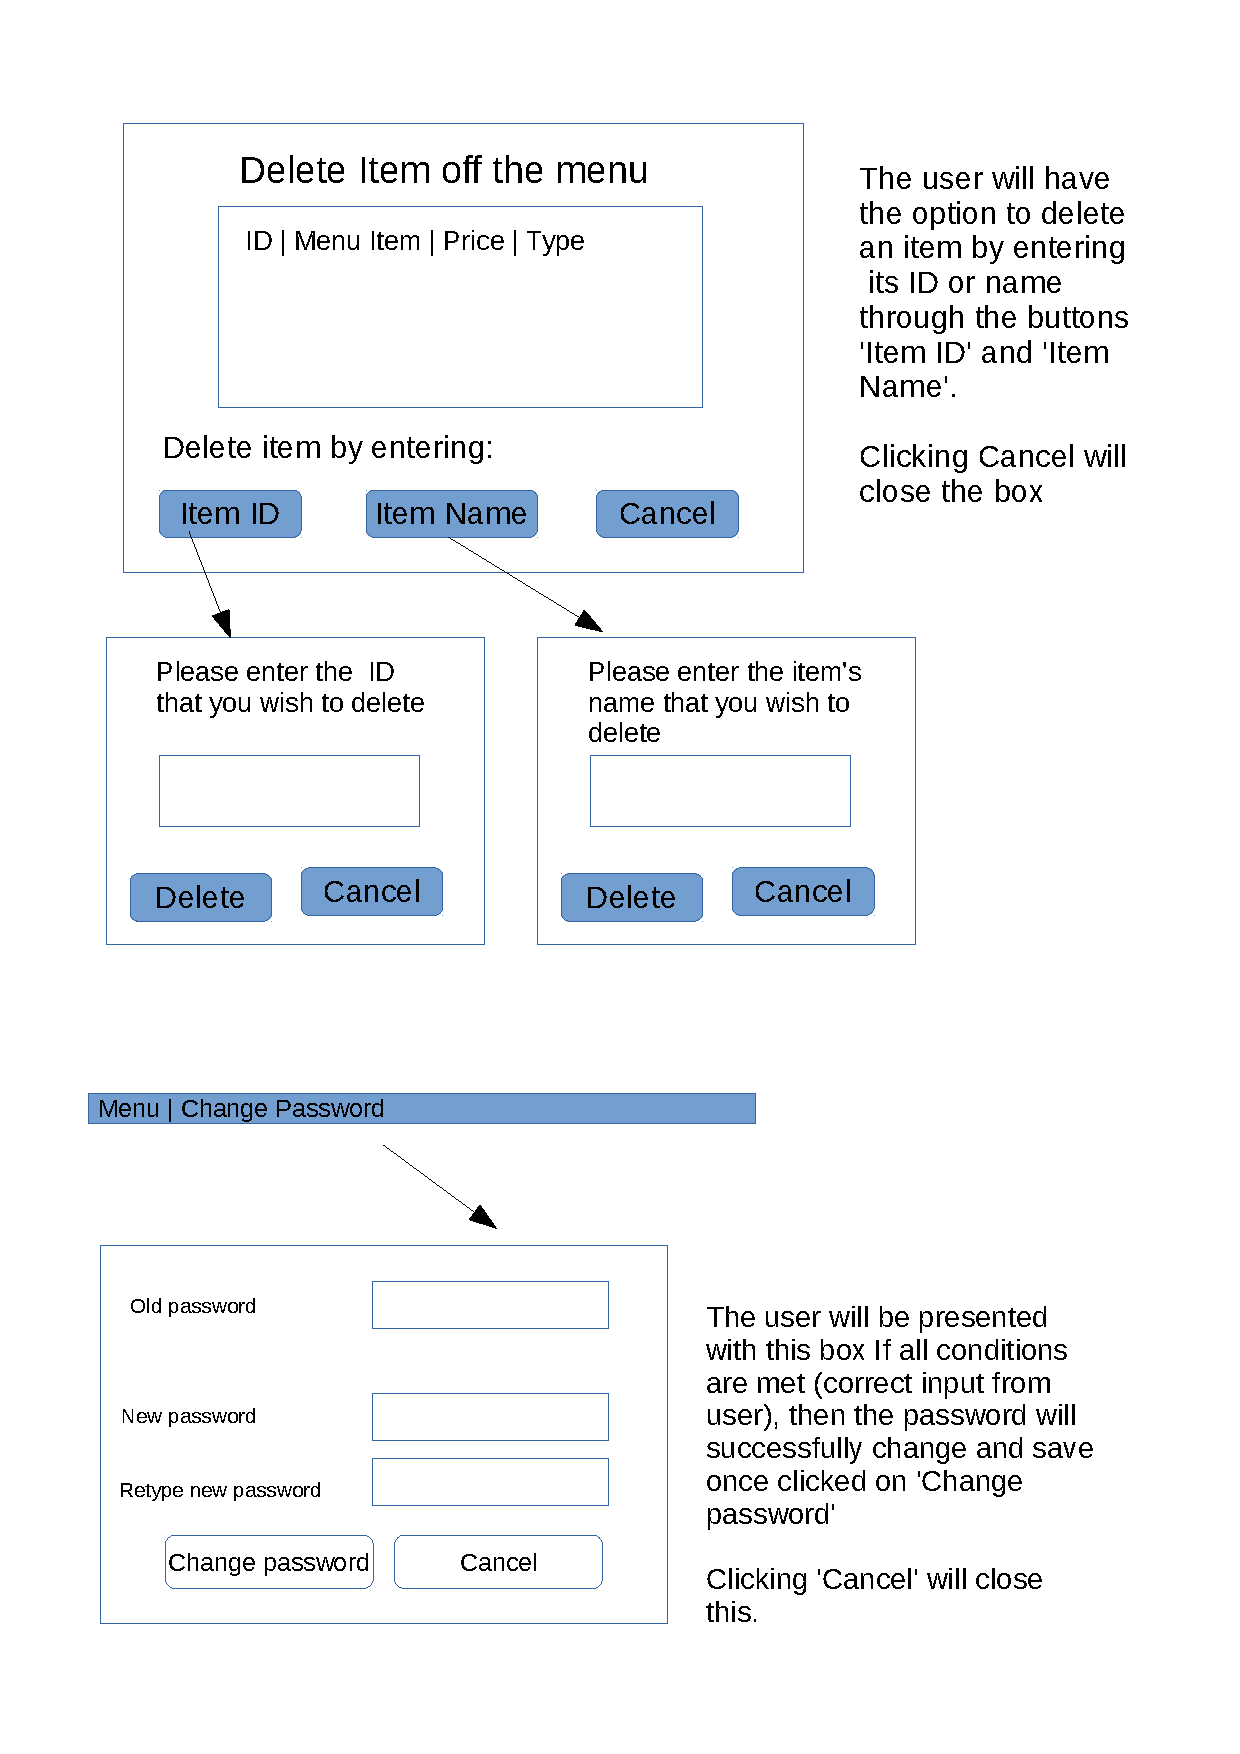
\includegraphics[height = 20cm]{./Design/Images/InterfaceMenuBar1}
    \caption{Explaining Menu Bar} \label{fig:MenuBar2}
\end{figure}

\begin{figure}[H]
    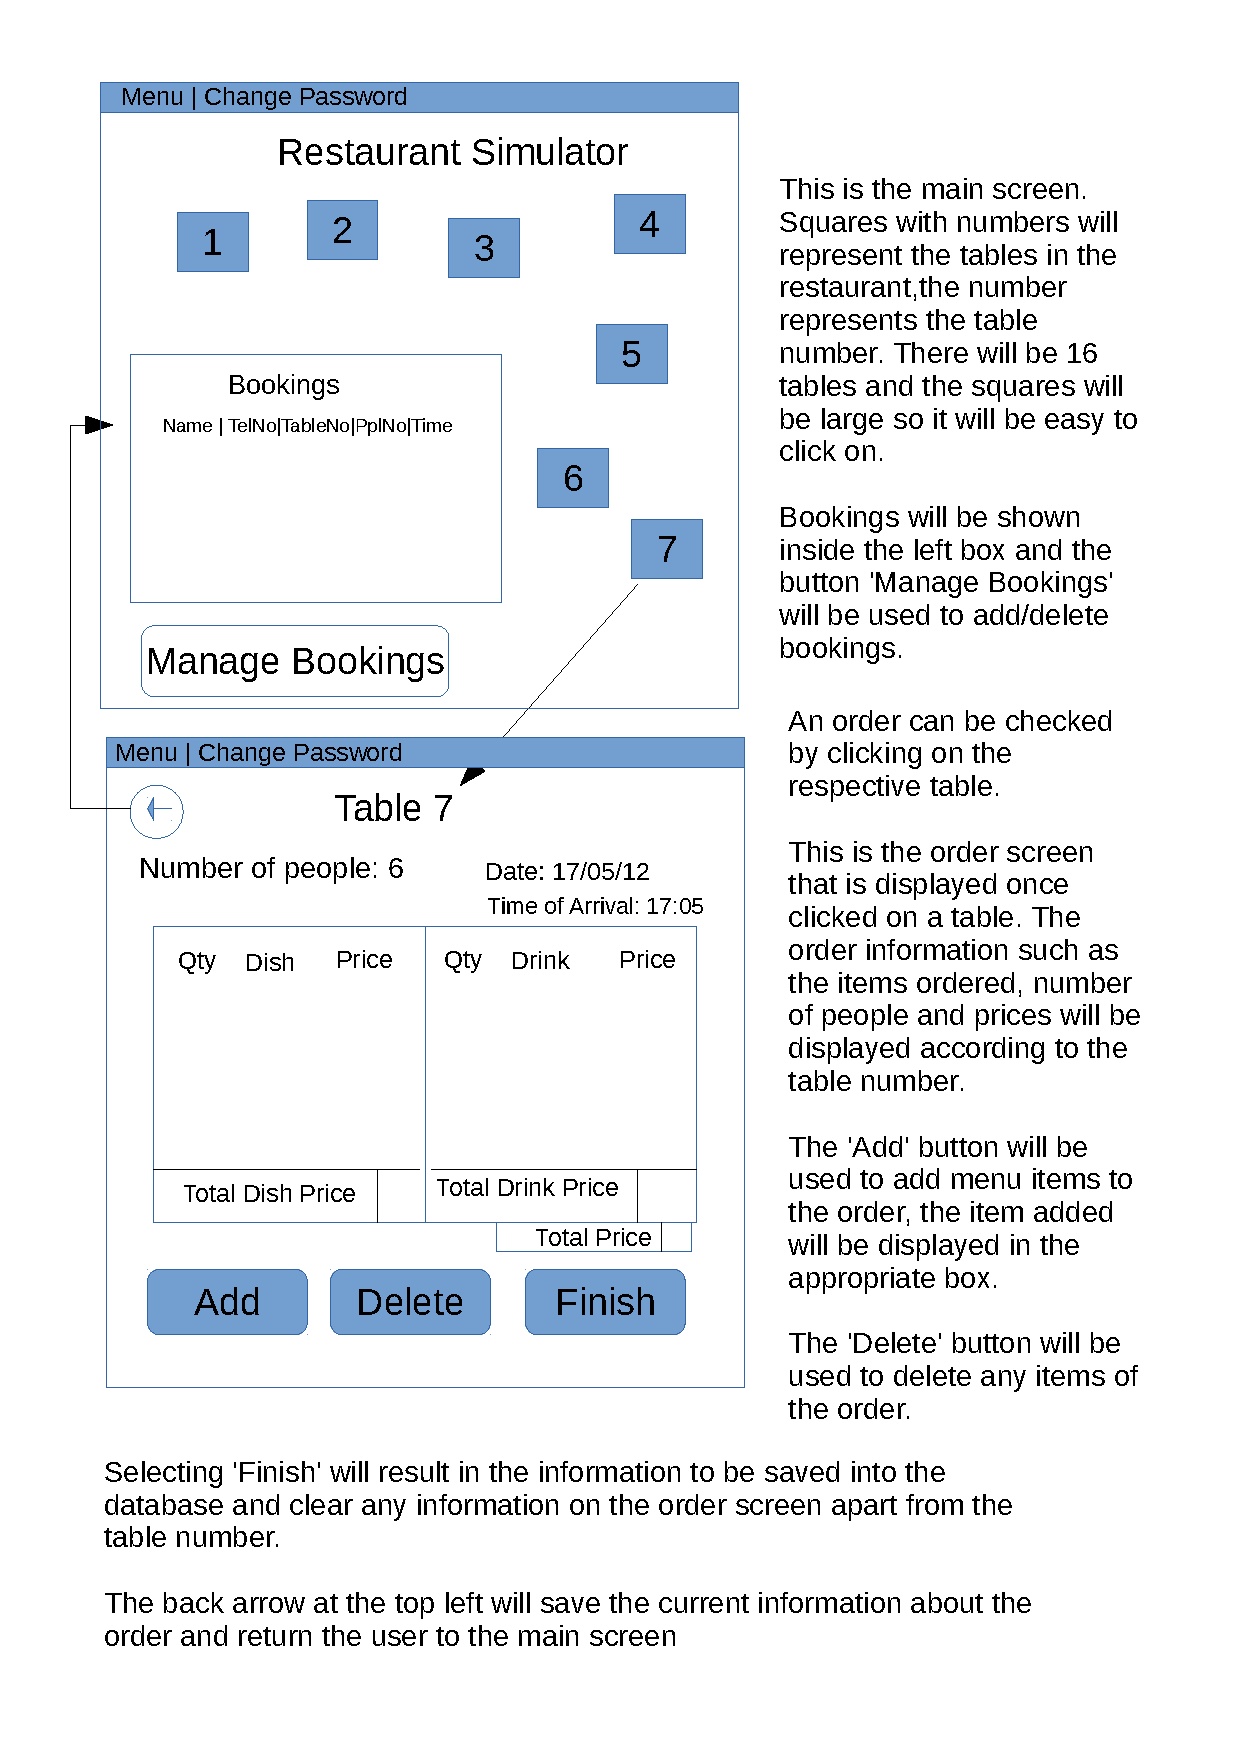
\includegraphics[height = 20cm]{./Design/Images/Interface2}
    \caption{Main Screen} \label{fig:Main}
\end{figure}


\begin{figure}[H]
    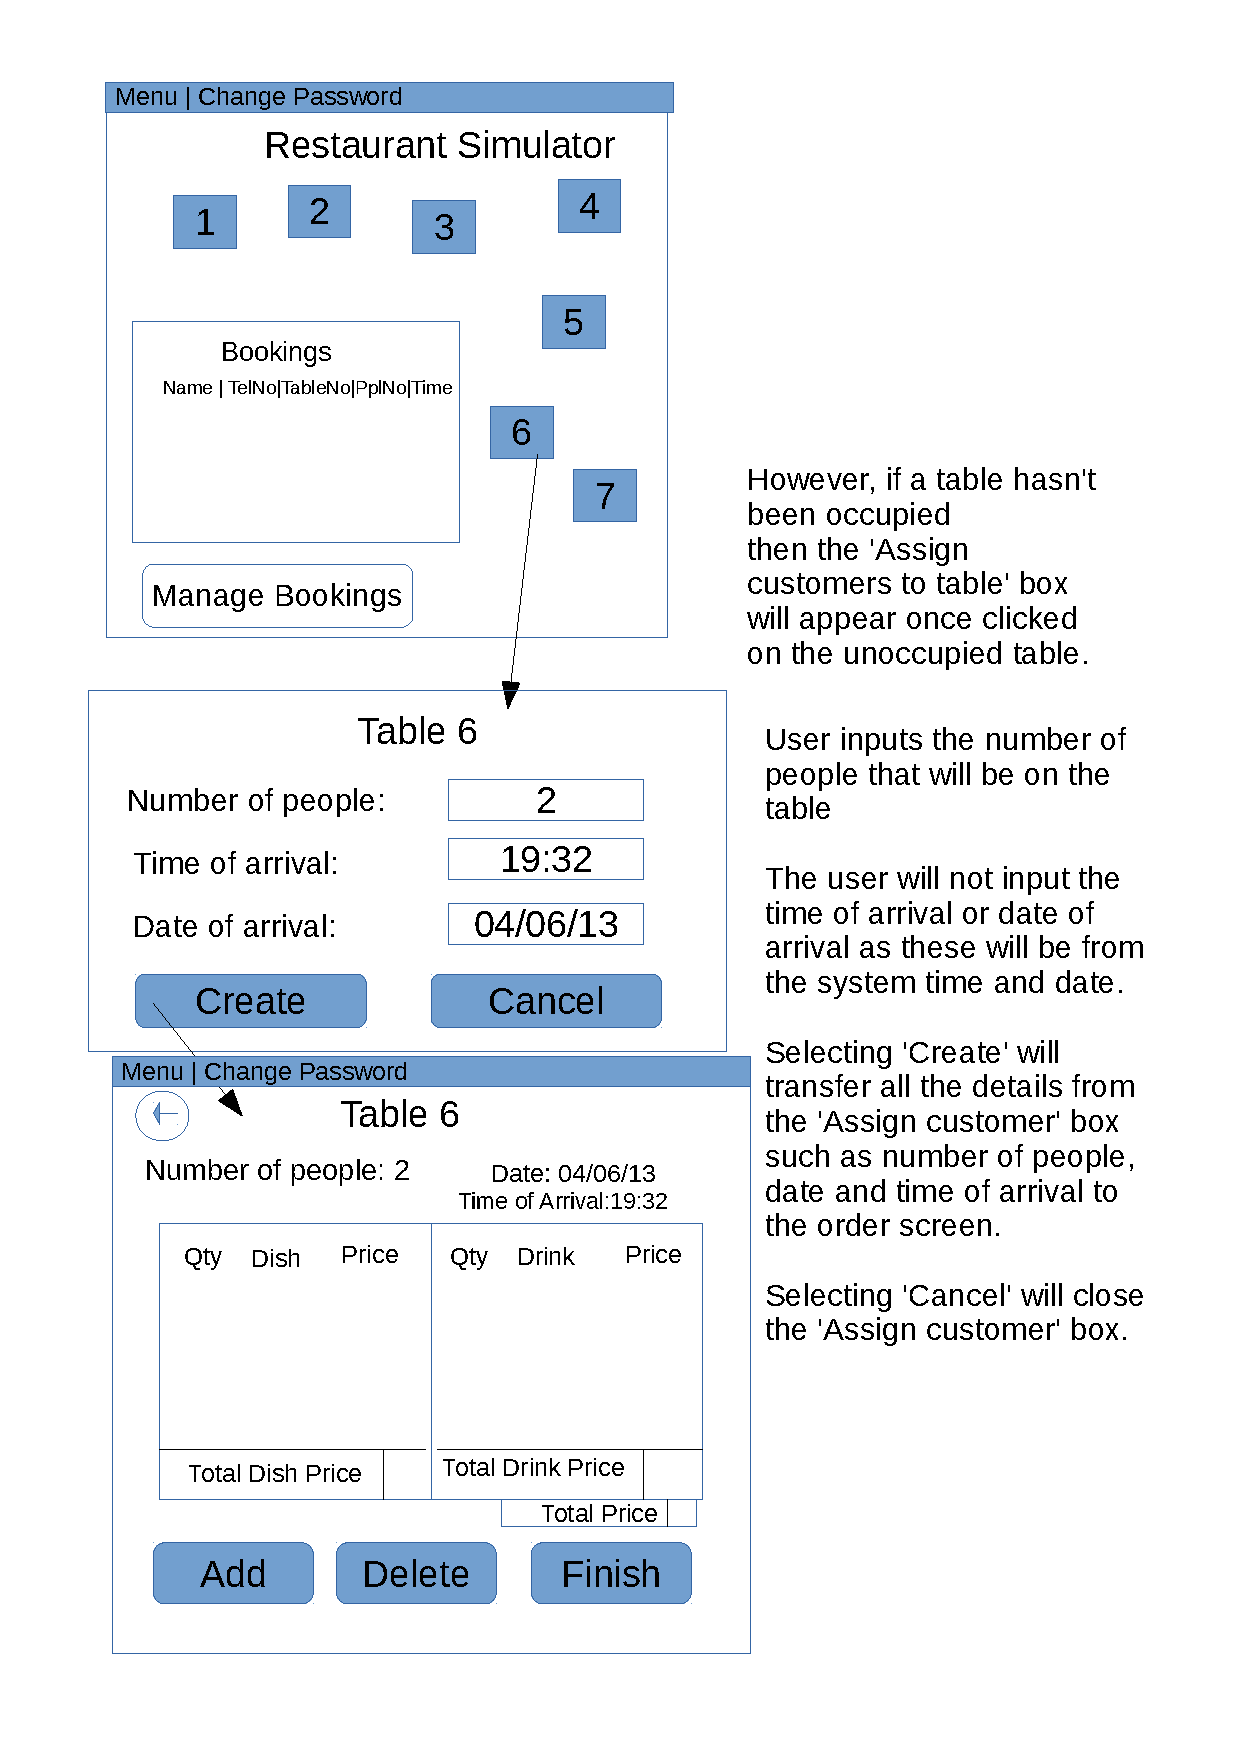
\includegraphics[height = 20cm]{./Design/Images/Interface7}
    \caption{Unoccupied table} \label{fig:UnocTable}
\end{figure}

\begin{figure}[H]
    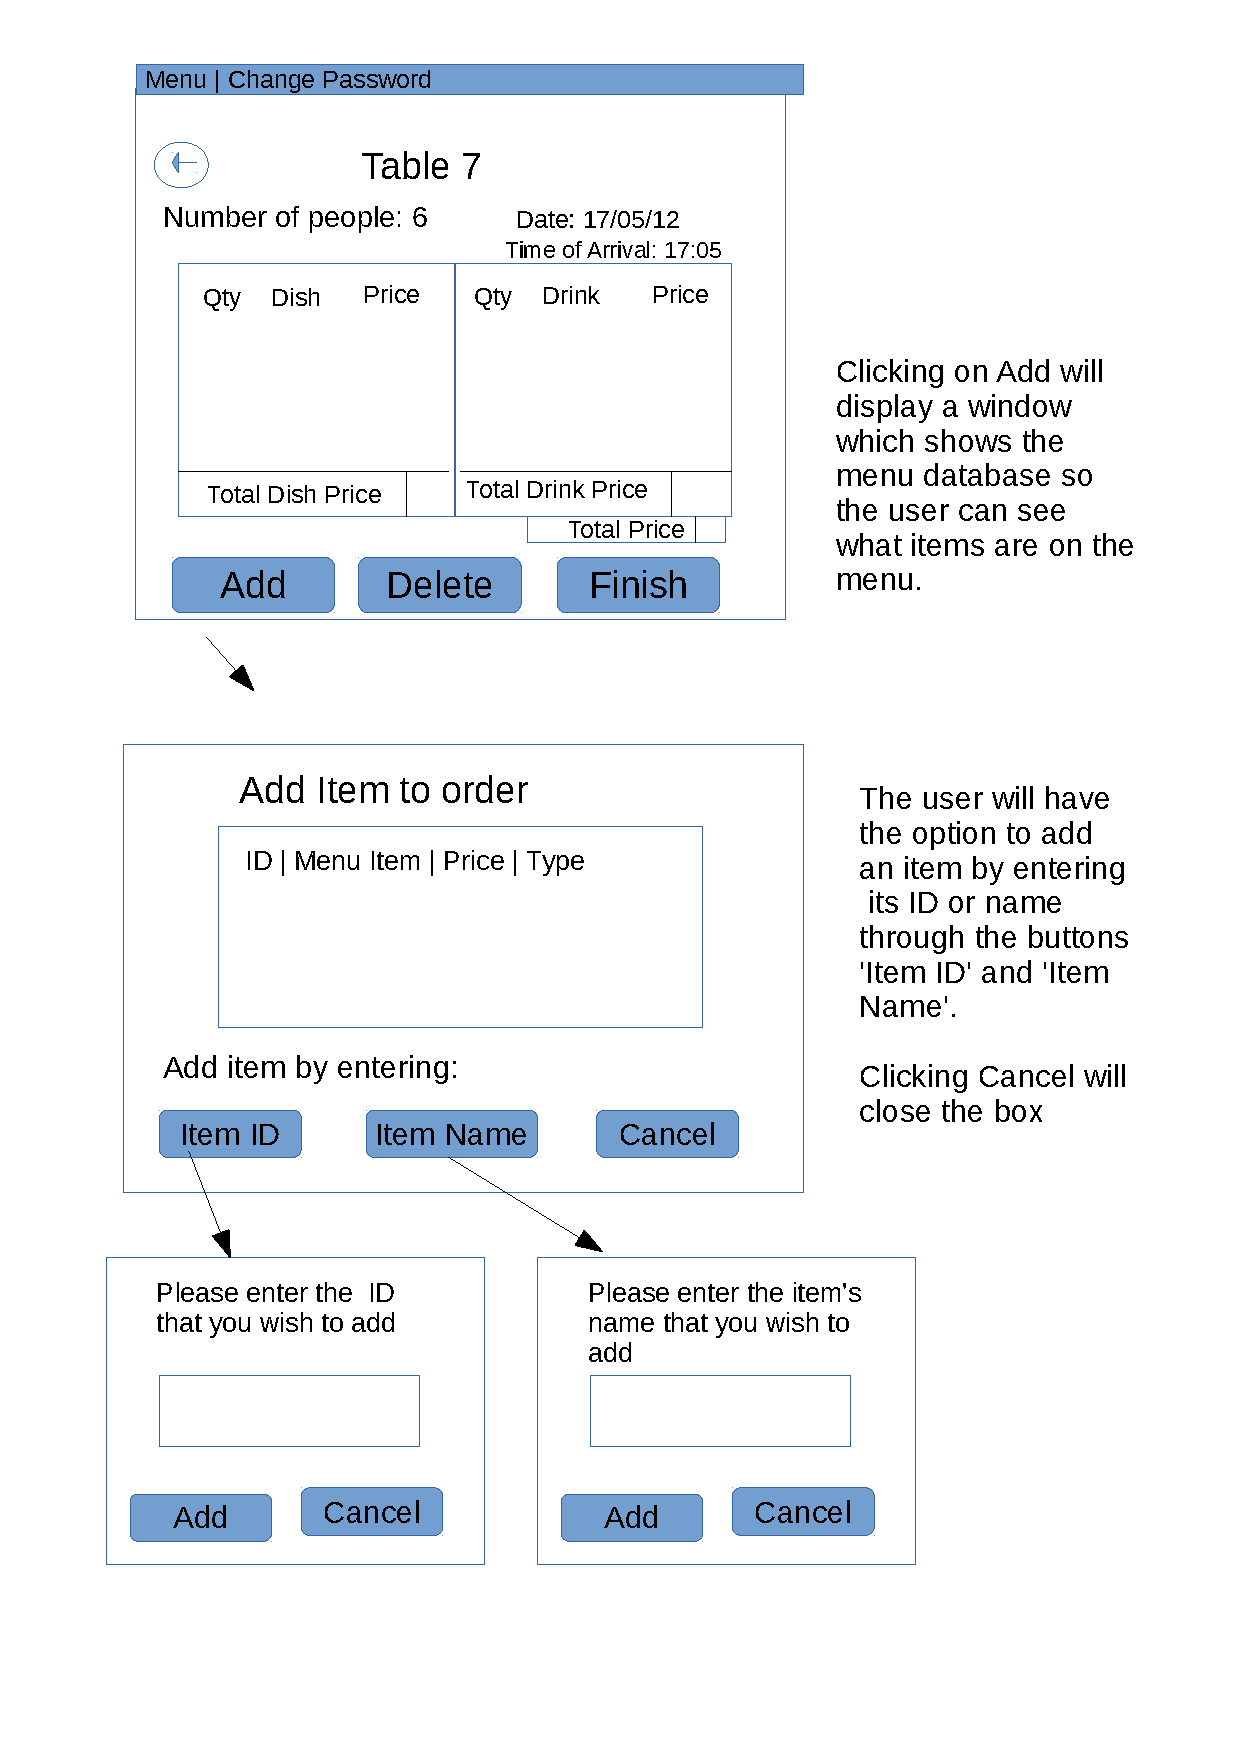
\includegraphics[height = 20cm]{./Design/Images/Interface3}
    \caption{Add Item} \label{fig:Add}
\end{figure}

\begin{figure}[H]
    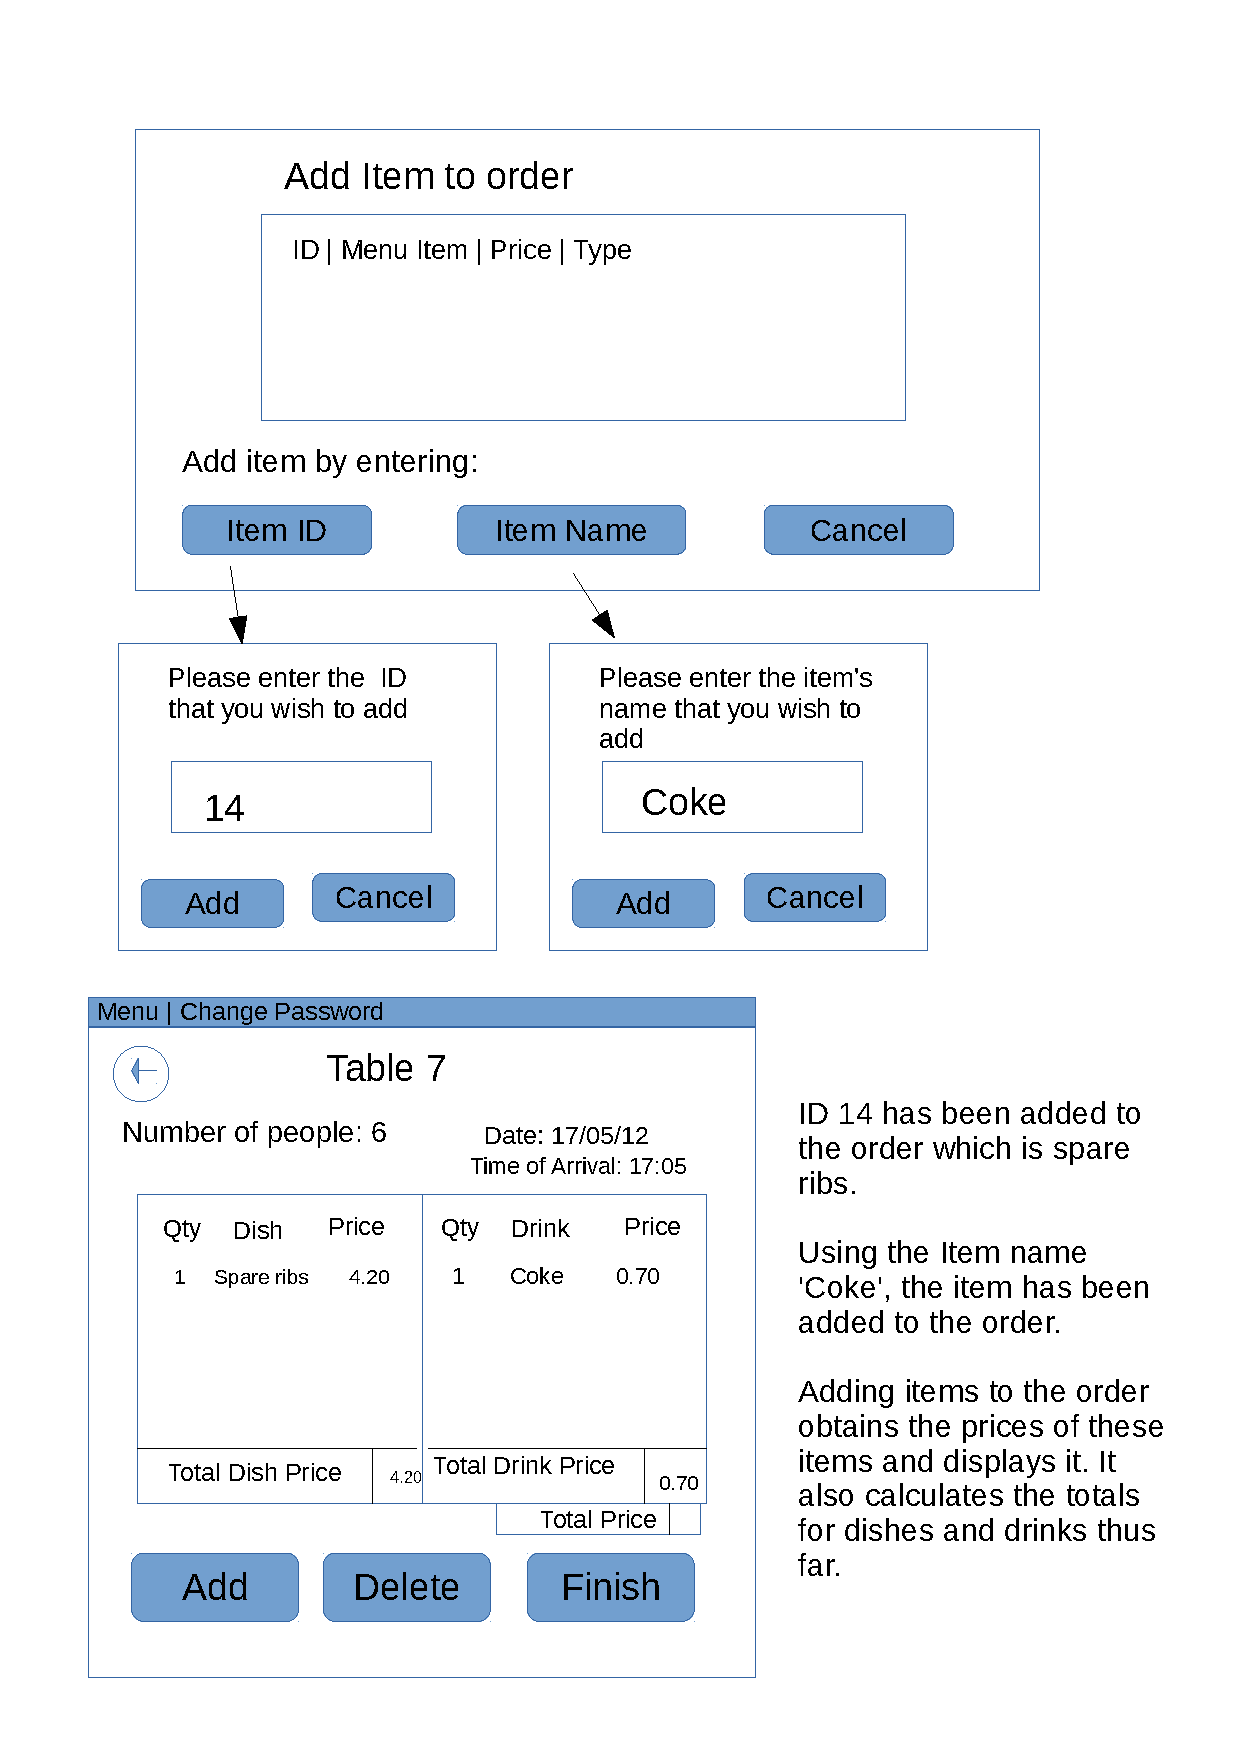
\includegraphics[height = 20cm]{./Design/Images/Interface33}
    \caption{Add Item} \label{fig:Adding}
\end{figure}

\begin{figure}[H]
    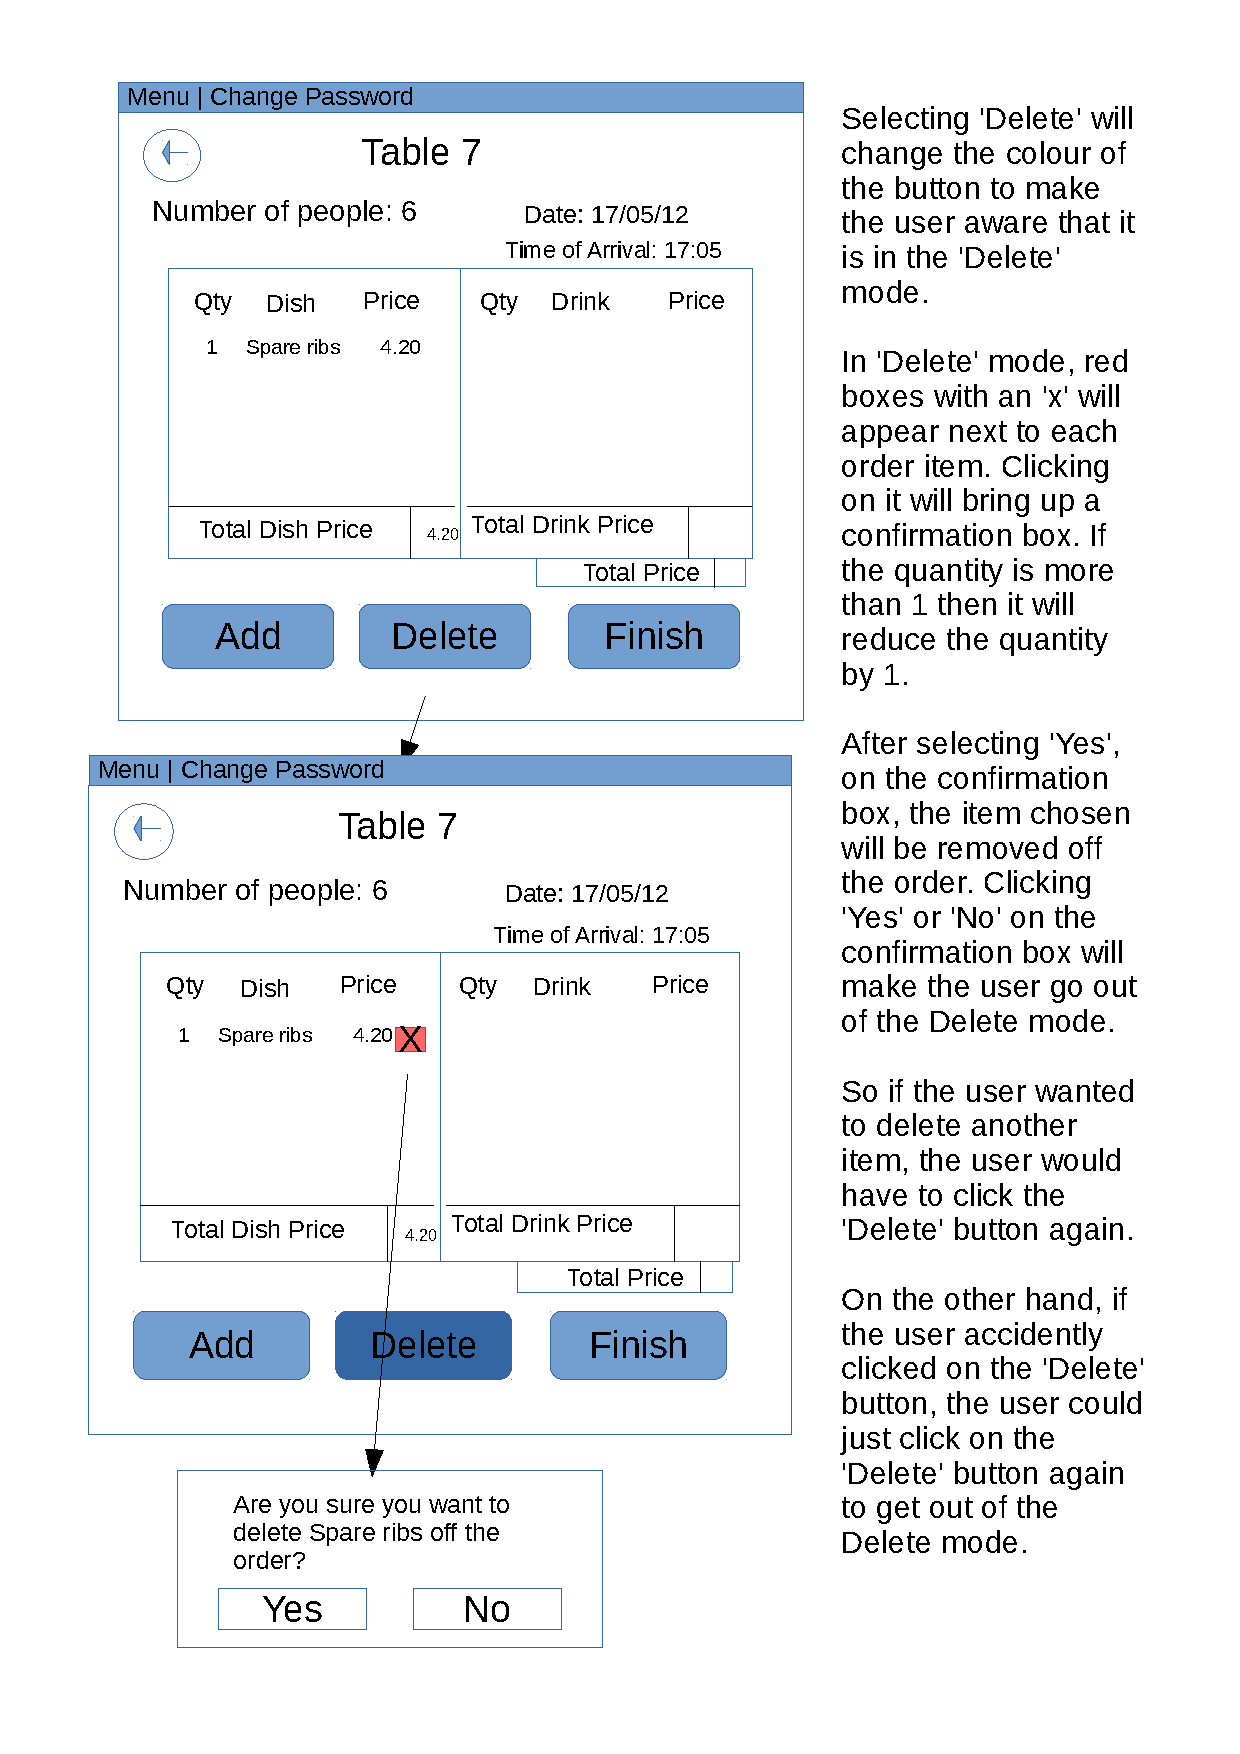
\includegraphics[height = 20cm]{./Design/Images/Interface4}
    \caption{Delete Item} \label{fig:Delete}
\end{figure}

\begin{figure}[H]
    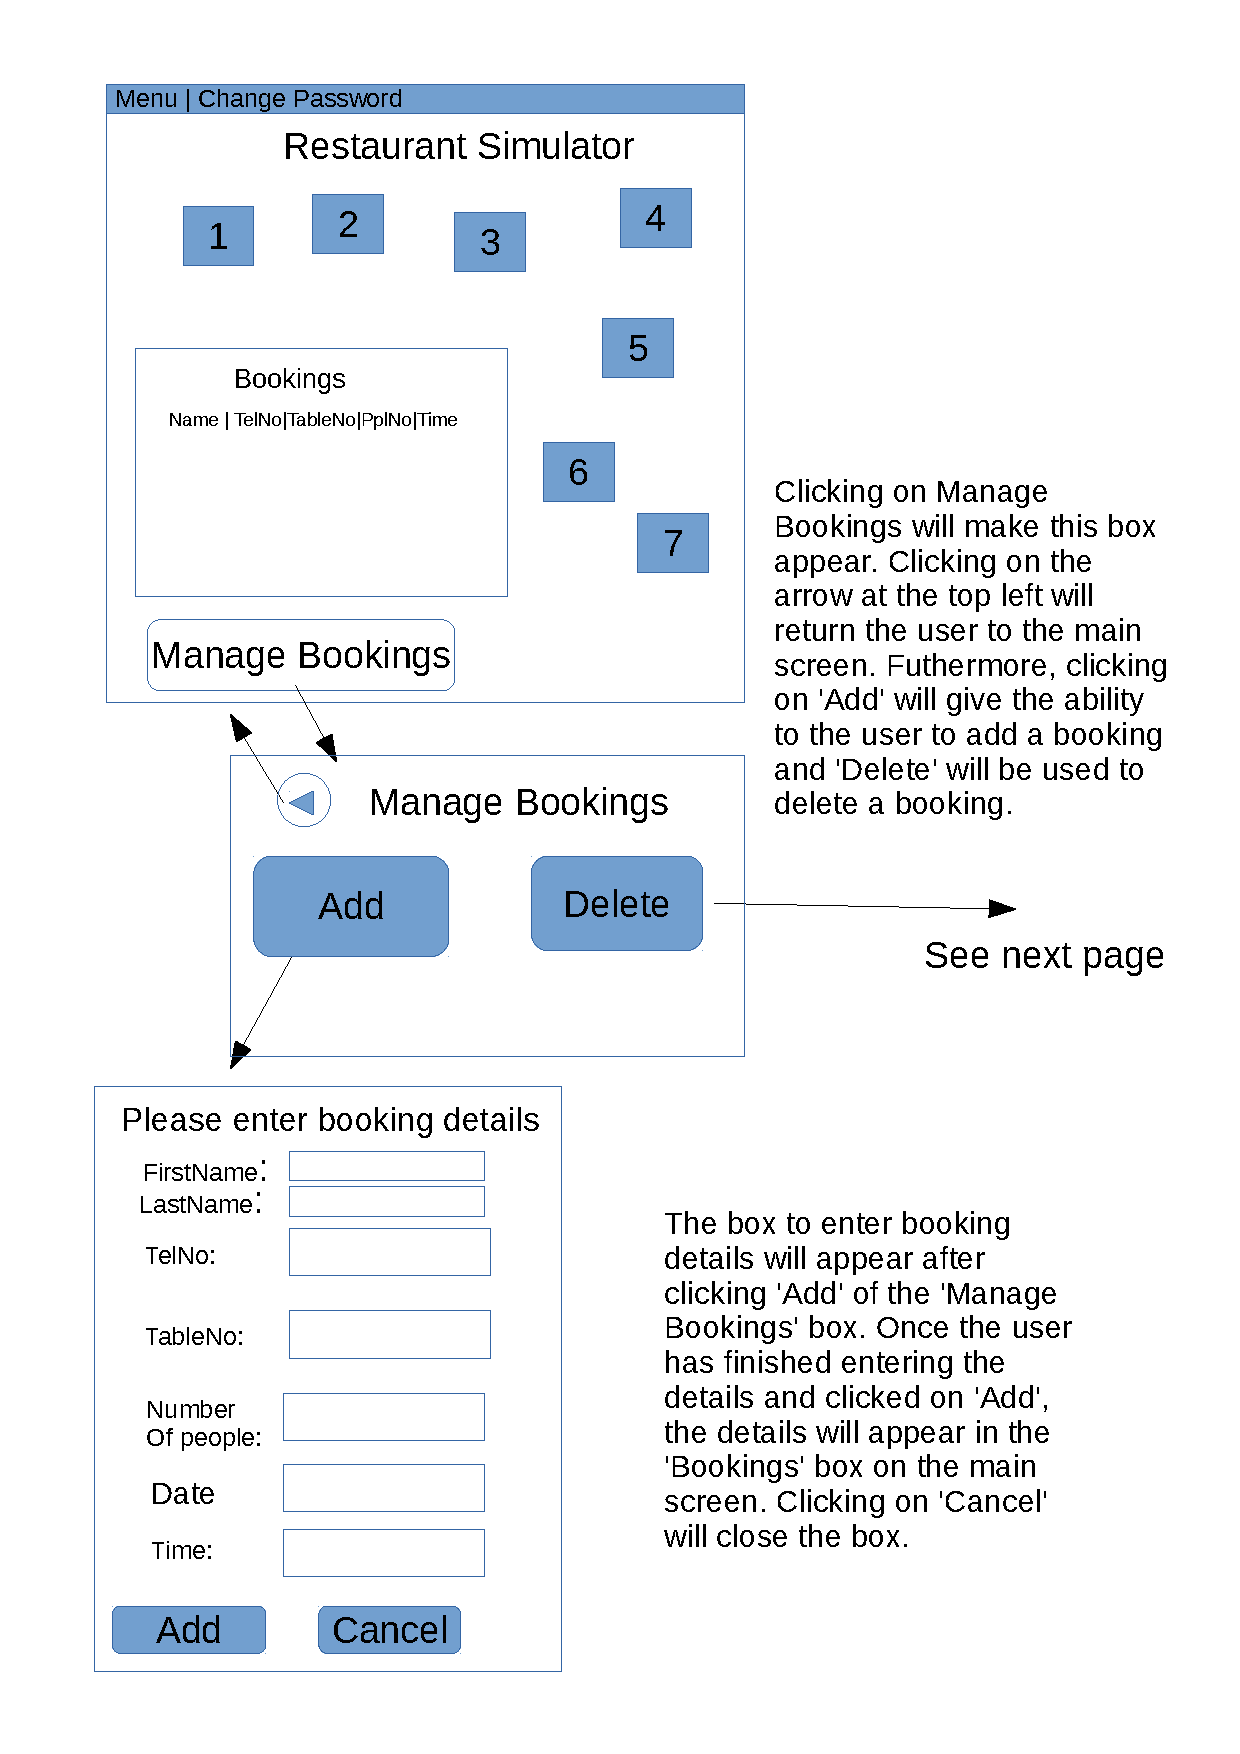
\includegraphics[height = 20cm]{./Design/Images/Interface5}
    \caption{Add Booking} \label{fig:Booking}
\end{figure}

\begin{figure}[H]
    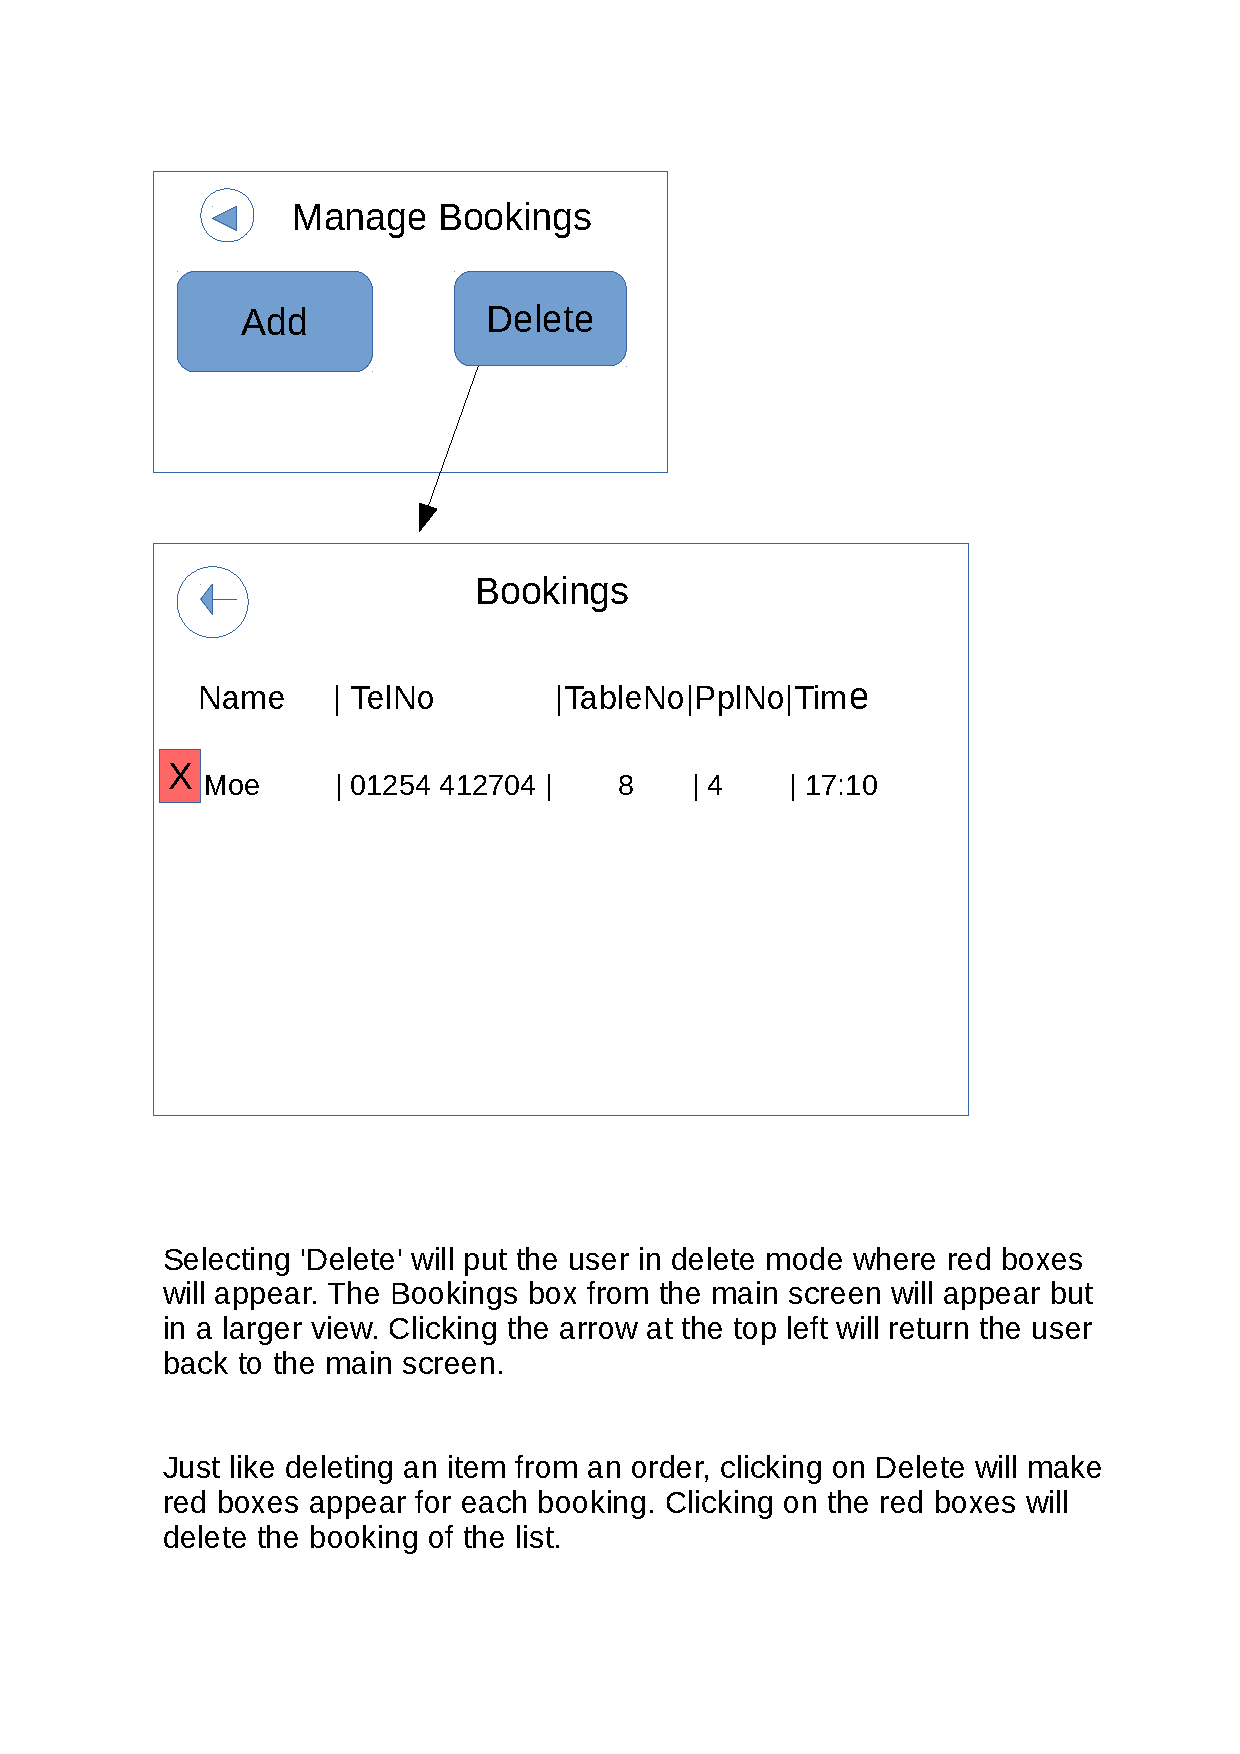
\includegraphics[height = 20cm]{./Design/Images/Interface6}
    \caption{Delete Booking} \label{fig:Booking2}
\end{figure}


\section{Hardware Specification}

Keyboard and mouse are essential as the keyboard will be used to input information and the mouse will be used to navigate. The program would need to fit a 19" screen, this is important because one of my client's main requirements is to be able to track information and so having a large window fitting the screen will make it easier to look at. A processer with 1GHz will be perfectly suitable for this program to run smoothly and since the user has AMD FX(fm) - 6300 six-core CPU 3.50GHz, the program shouldnt run without any problems. In addition, not much RAM would be needed to run this program, 1GB would be more than enough and since the user has 8GB RAM the program shouldn't experience any further hardware based problems.
\section{Program Structure}

\subsection{Top-down design structure charts}

\begin{figure}[H]
    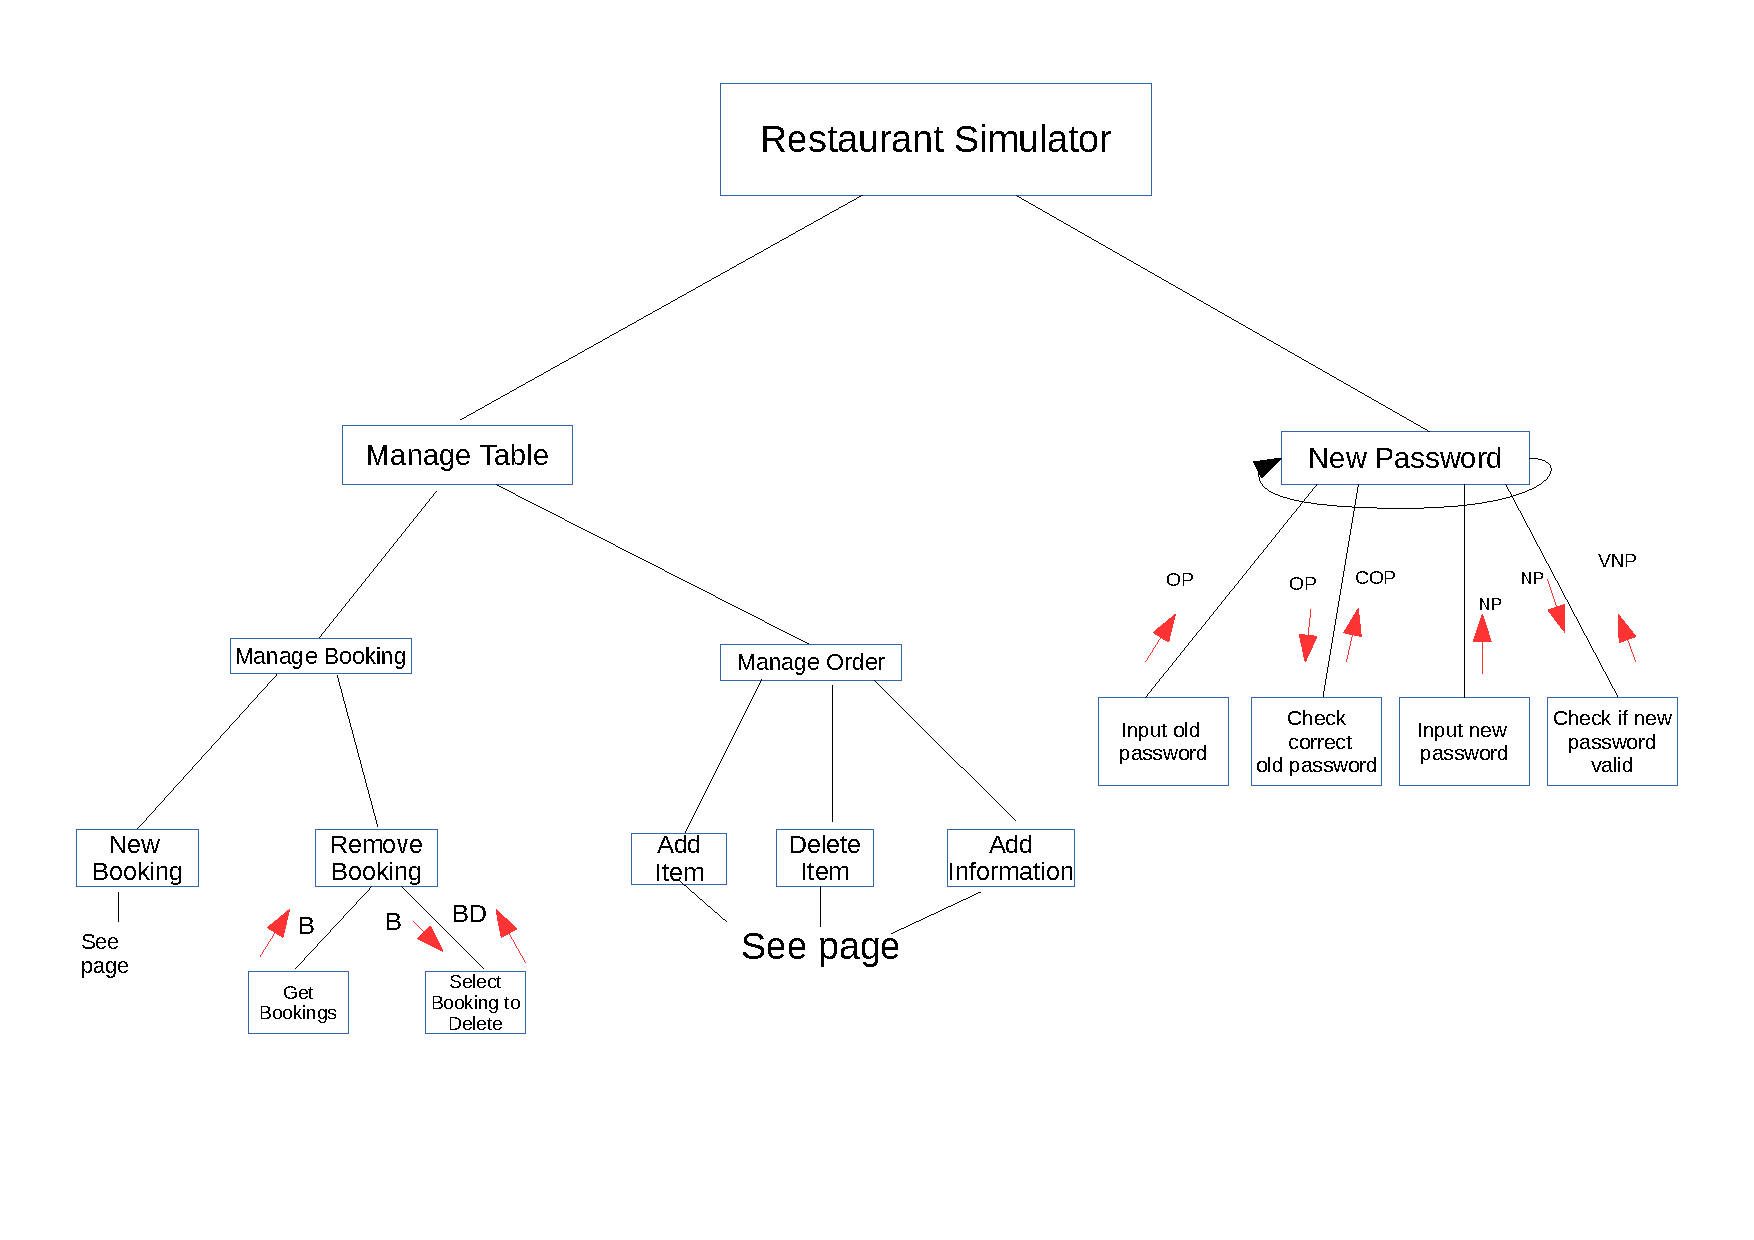
\includegraphics[height = 12cm, angle = -90]{./Design/Images/structure1}
    \caption{Main structure} \label{fig:Structure1}
\end{figure}

\begin{figure}[H]
    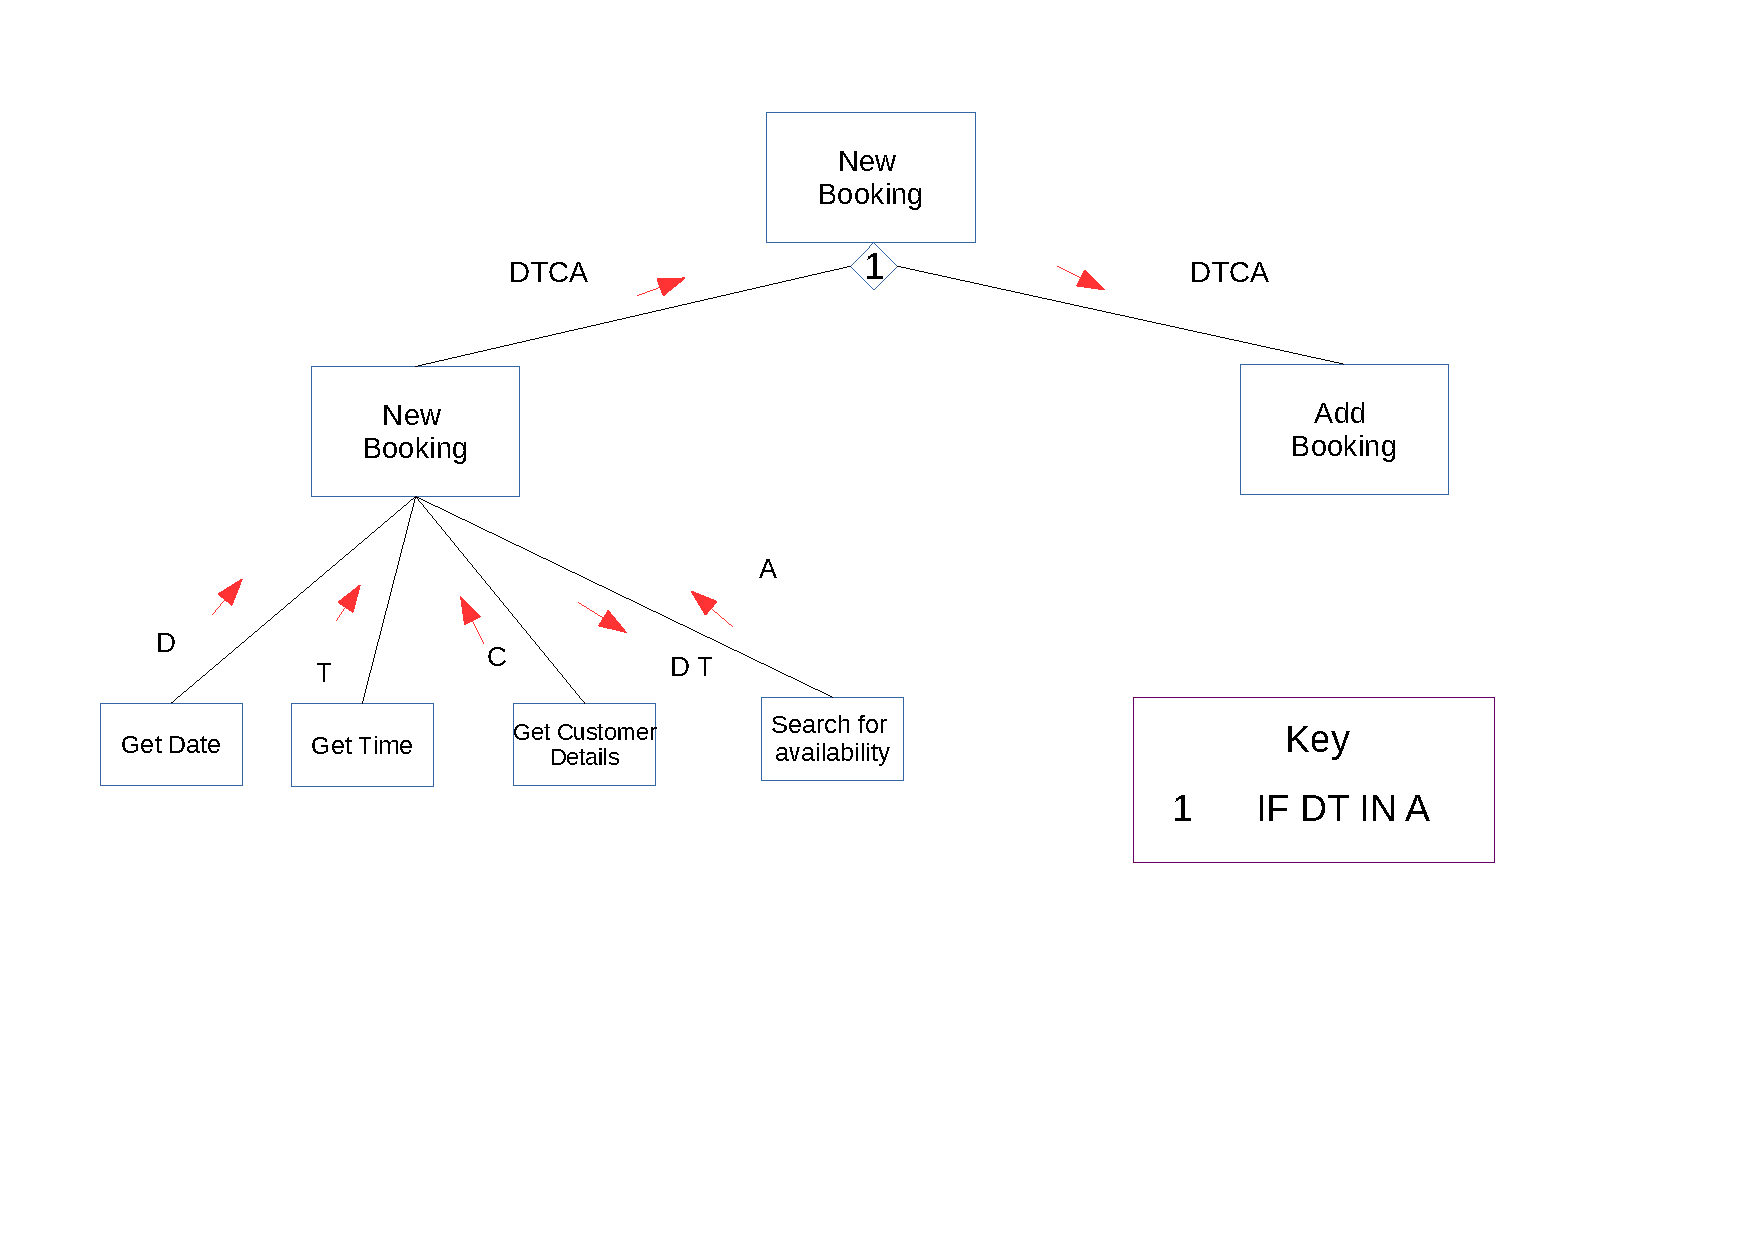
\includegraphics[height = 15cm, angle = -90]{./Design/Images/structure2}
    \caption{Add Booking Structure} \label{fig:Structure2}
\end{figure}

\begin{figure}[H]
    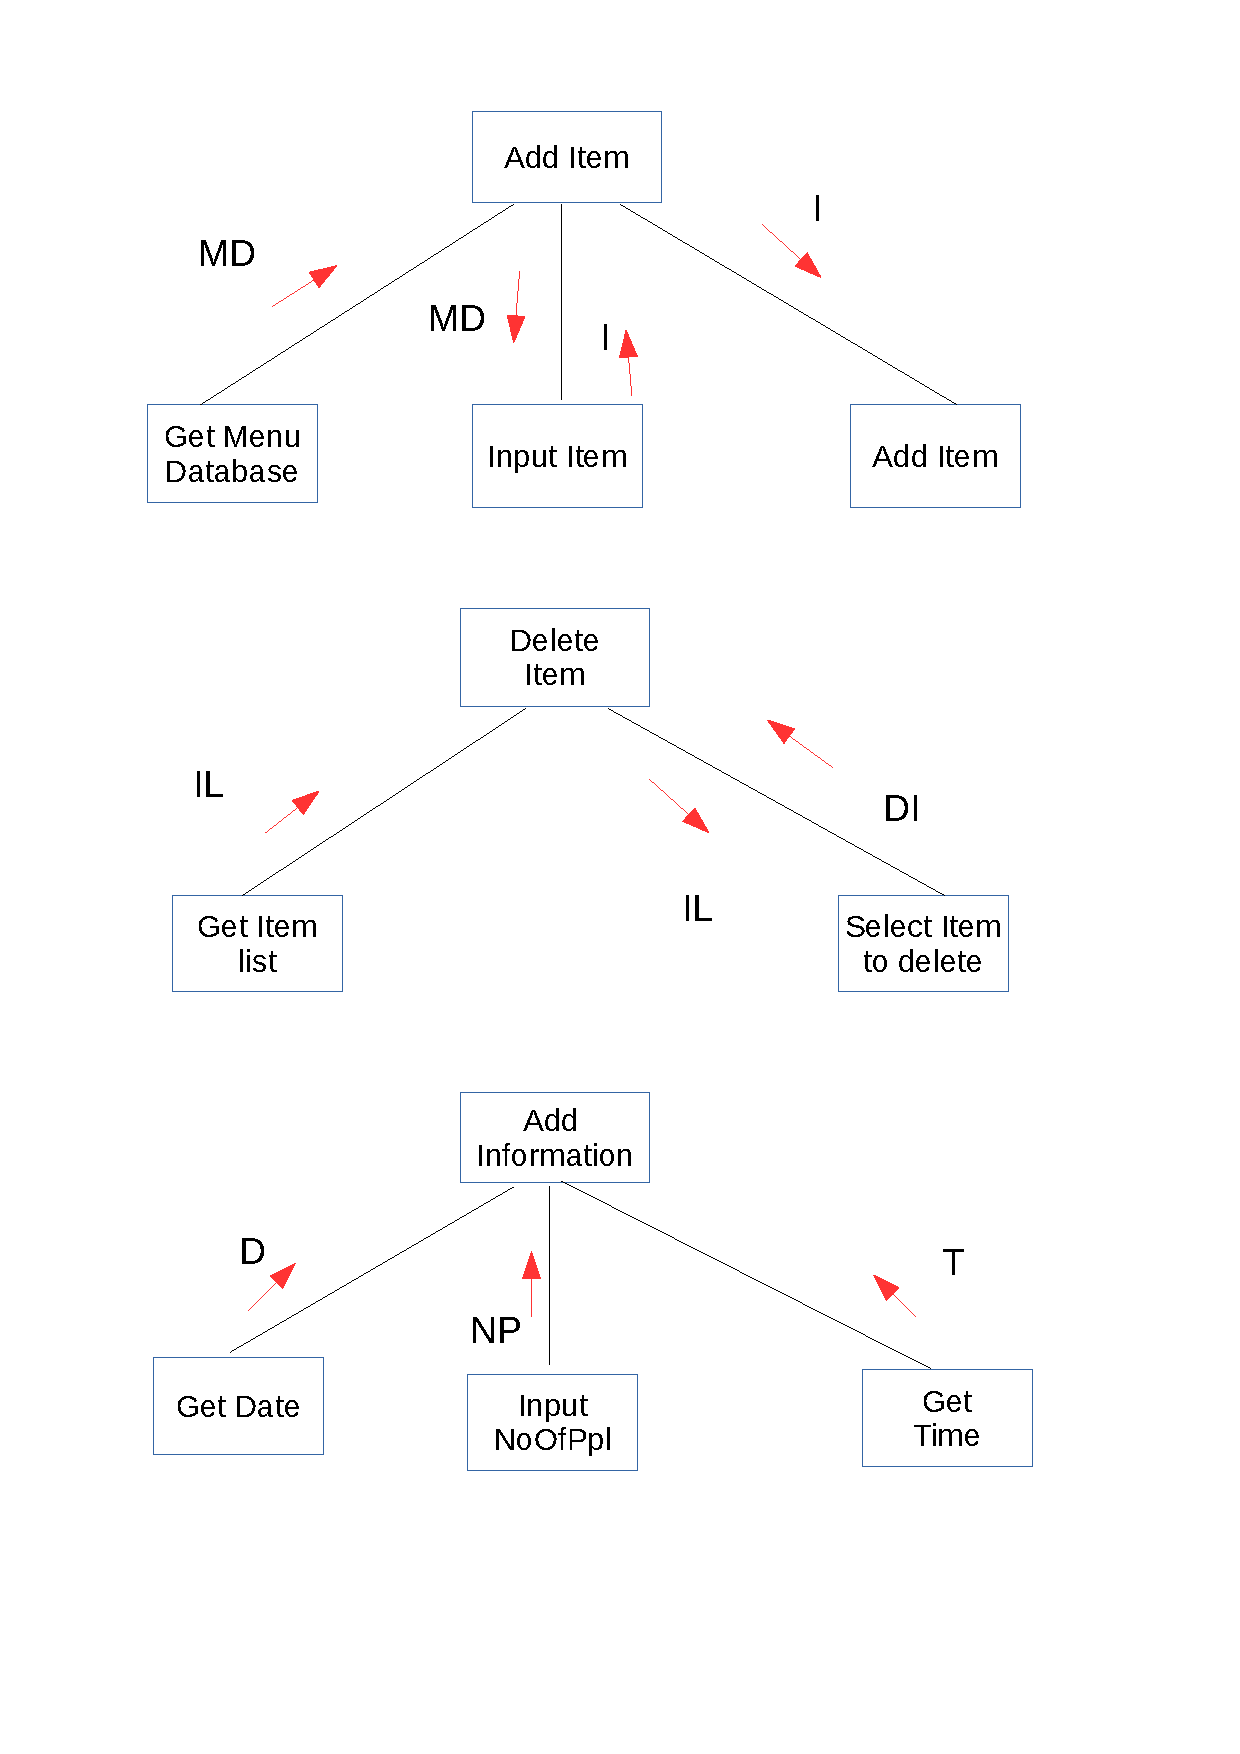
\includegraphics[height = 20cm]{./Design/Images/structure3}
    \caption{Editing Order} \label{fig:Structure3}
\end{figure}

\subsection{Algorithms in pseudo-code for each data transformation process}


\begin{algorithm}[H]
\label{fig:repeat_as_while_pseudo_example_2}
    \caption{Password change}
\begin{algorithmic}[1]
\SET{$Old Password$}{$CurrentPassword$}
\SET{$ValidNewPassword$}{$False$}

\State
\SEND{$"Please \ enter \ the \ old \ password"$}
\RECEIVE{$UserCurrentPassword"$}
\State
\If {$UserCurrentPassword = OldPassword$}

	\While{$not ValidNewPassword$}
	\SEND{$"Please\ enter\ a\ new\ password (Must \ be \ longer \ than \ 4 \ characters)"$}
	\RECEIVE{$NewPassword$}
	\SEND{$"Please\ re-enter\ the \ new \ password"$}
	\RECEIVE{$ReEnteredNewPassword$}
	\If{$ len(NewPassword)>4 \ AND \ NewPassword = ReEnteredNewPassword$}
    		\SET{$CurrentPassword$}{$NewPassword$}
		\SET{$ValidNewPassword$}{$True$}		
	\Else
		\SEND{$Please \ try \ again.$}

	\EndIf

\EndWhile
\State
\Else
	\SEND{$You \ have \ entered \ the \ wrong \ password.$}

\EndIf
\end{algorithmic}
\end{algorithm}		

\begin{algorithm}[H]
\label{fig:AddPseudo}
    \caption{Adding an item to an order(MenuID database will need to be retrieved)}
\begin{algorithmic}[1]

\State

    \SEND{$"Please\ enter\ a\ menuID"$}
    \RECEIVE{$GetMenuID$}
\If{$GetMenuID \ in \ MenuID \ Database$}
    \SET{$ItemAdded$}{$(MenuIDDatabase \ ,MenuItems$}
	
	OrderList.insert(ItemAdded)
\Else
	\SEND{$You \ have \ entered \ an \ invalid \ menuID$}
\EndIf
\end{algorithmic}
\end{algorithm}

\begin{algorithm}[H]
\label{fig:repeat_pseudo_example}
    \caption{Calculating prices}
\begin{algorithmic}[1]
\SET{$TotalPrice$}{$0$}
\SET{$OrderLength$}{$Length(OrderedItems)$}


\State
	\For {$OrderedItems.Price$}{1}{$OrderLength$}
		\SET{$TotalPrice$}{$TotalPrice+OrderedItems.Price$}
	\EndFor

\end{algorithmic}
\end{algorithm}

\subsection{Object Diagrams}

\begin{figure}[H]
    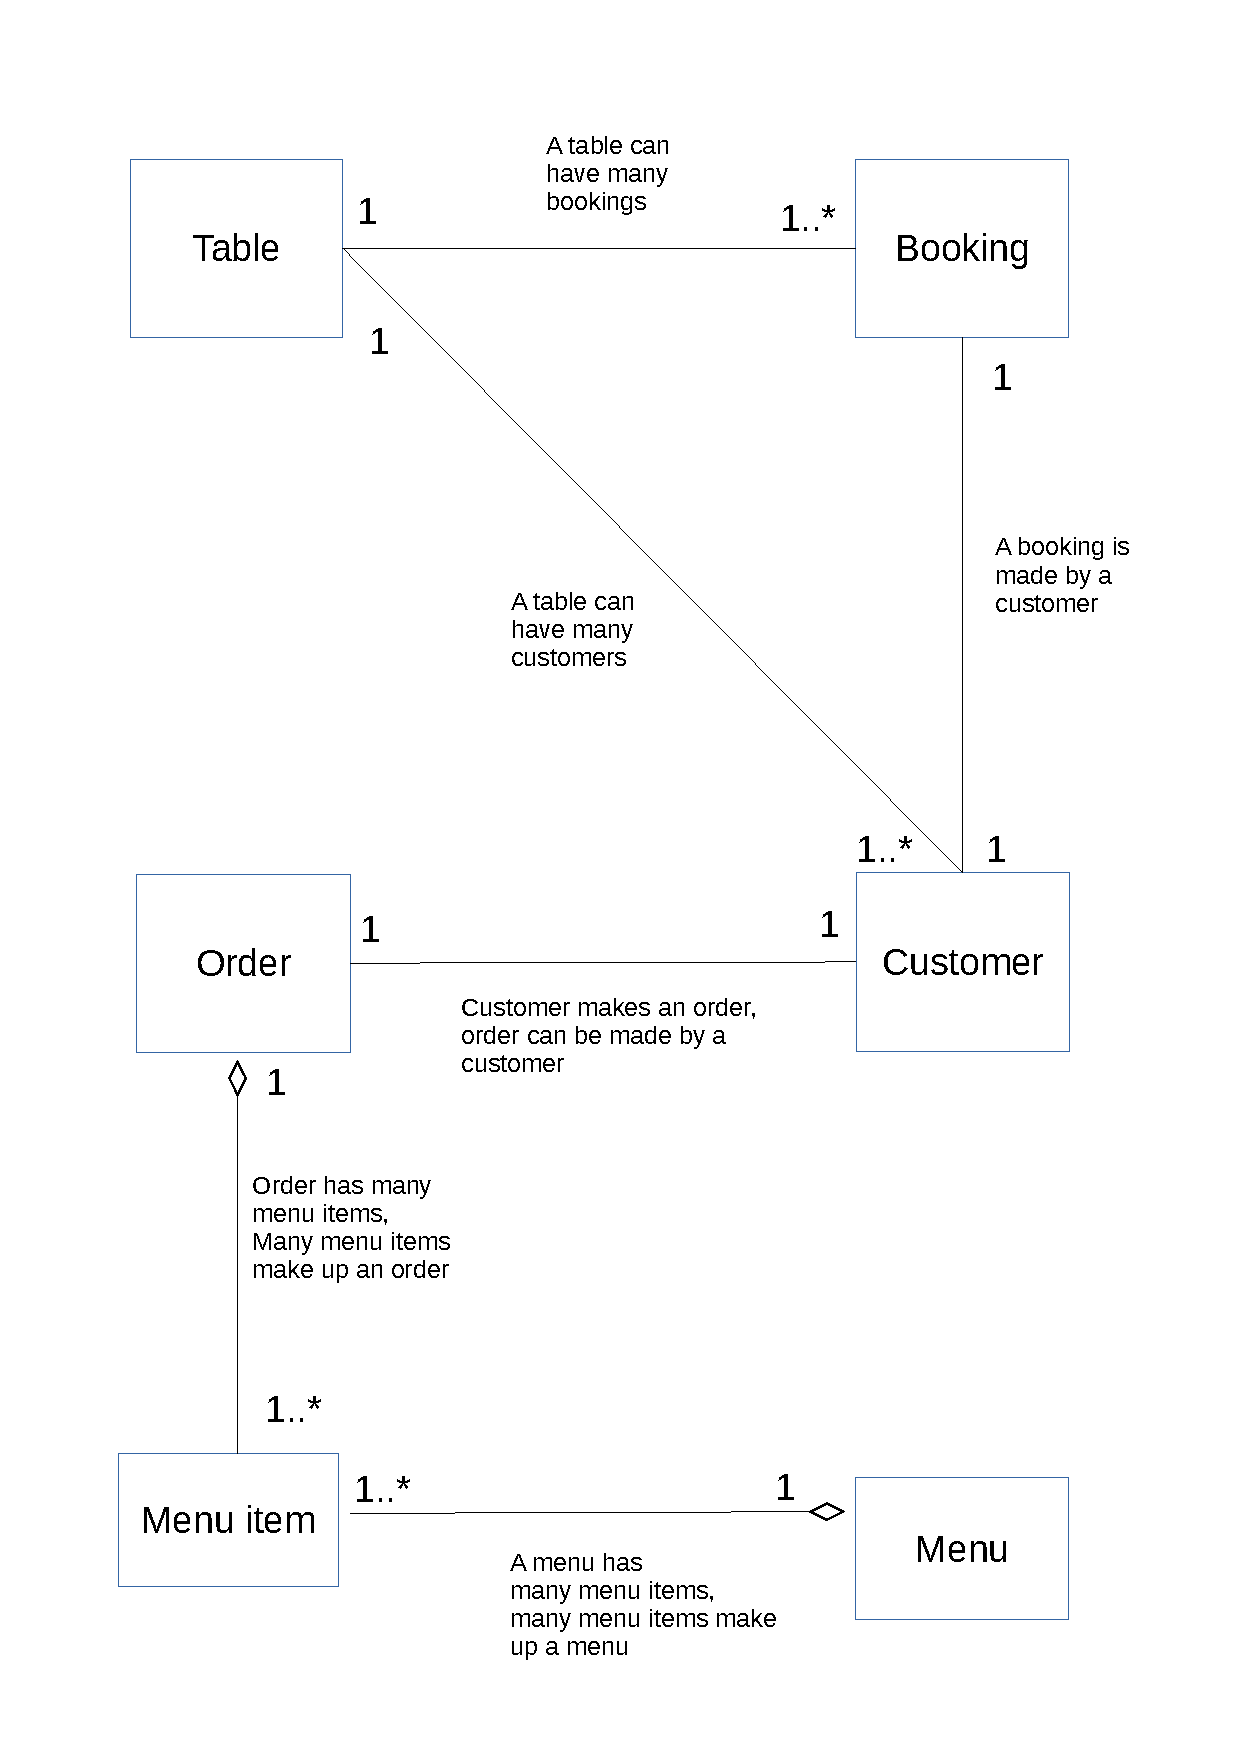
\includegraphics[height = 20cm]{./Design/Images/Objects2}
    \caption{Object Diagram} \label{fig:ObjectsD}
\end{figure}


\subsection{Class Definitions}

\begin{figure}[H]
    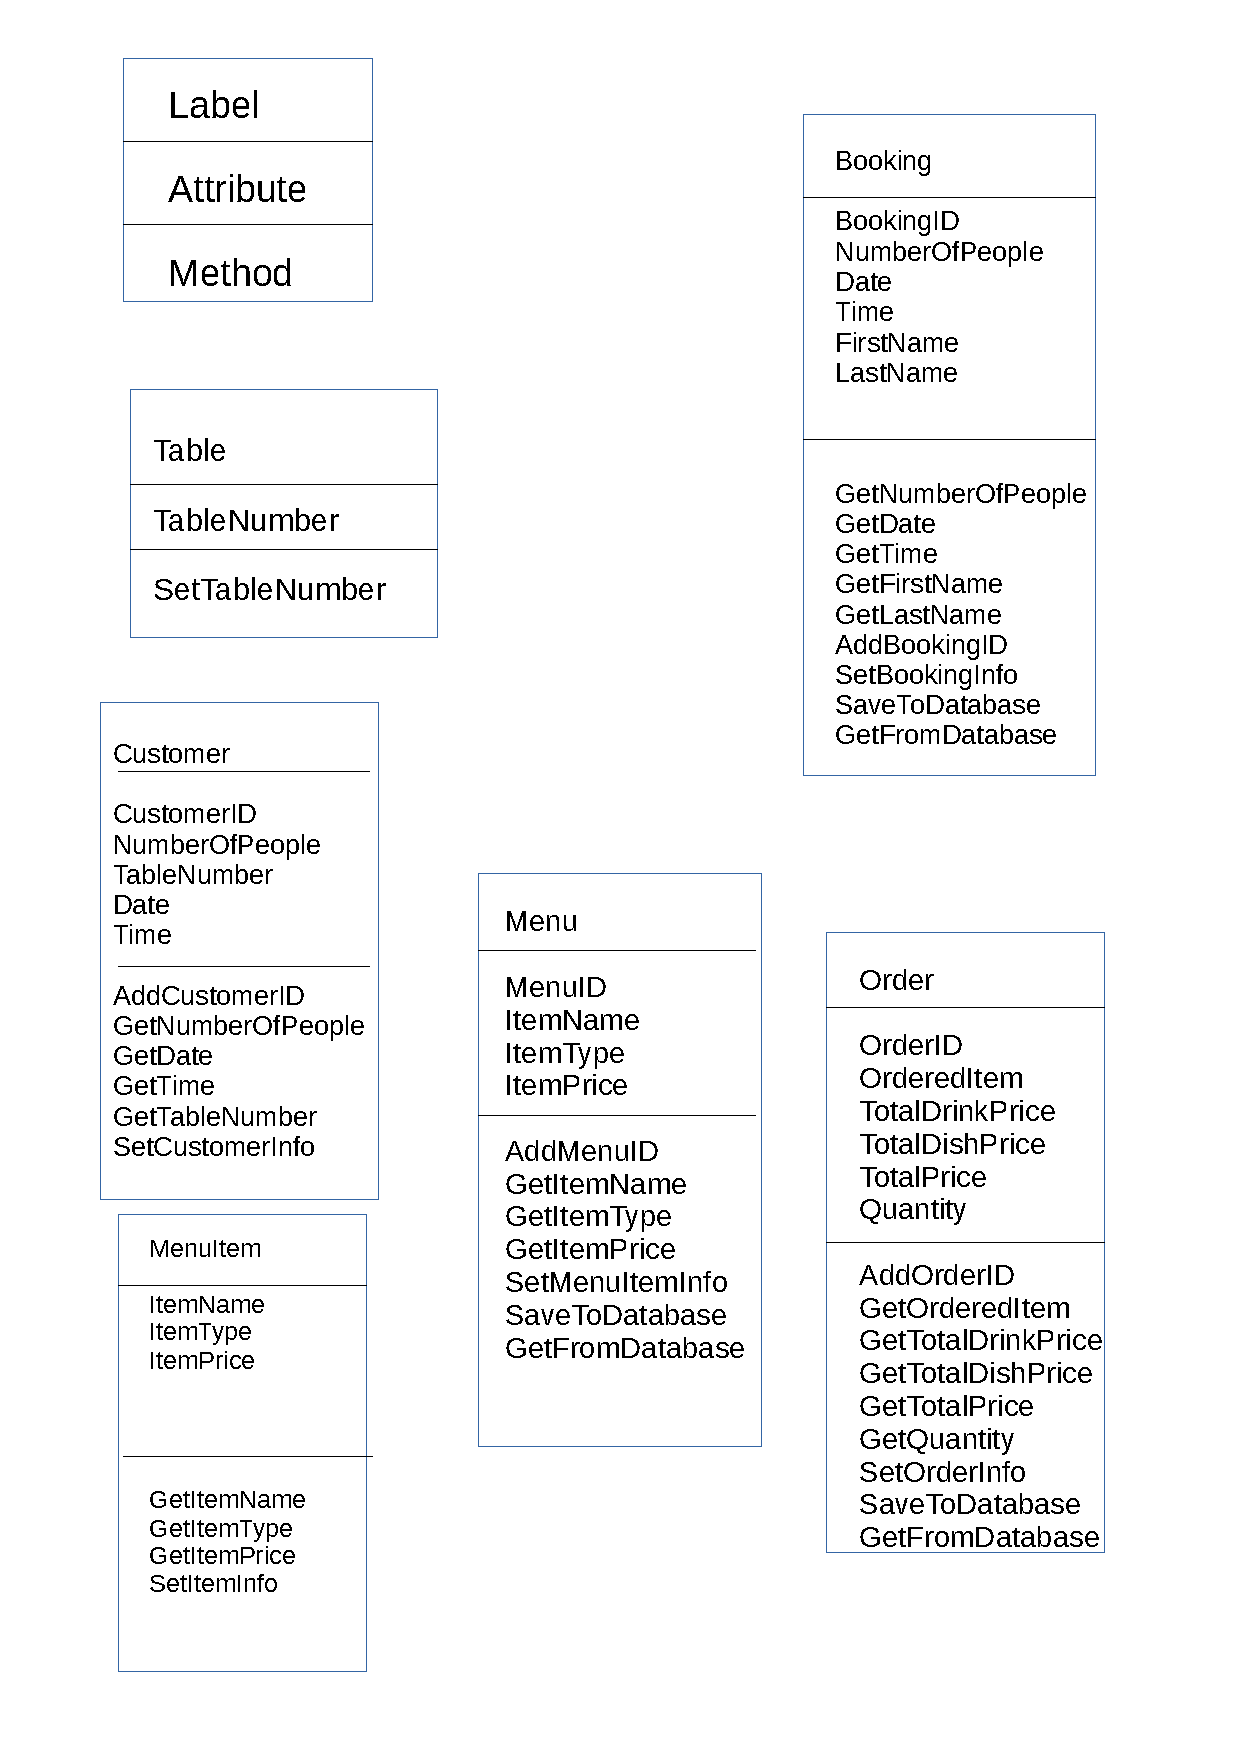
\includegraphics[height = 20cm]{./Design/Images/ClassDefinitions}
    \caption{Class Definitions} \label{fig:ClassD}
\end{figure}

\section{Prototyping}

There are many parts of the system that I would like to prototype due to my limited knowledge of them or its complexity.  

I will try to prototye:

\begin{itemize}

	\item The graphical user interface as this would probably one of the most difficult parts of the system I have to create due to not having a lot of experience in the area.
	\item Linking tables to the correct current customer order through GUI. By linking, I want it to display all the correct information such as what they ordered.
	\item The order screen where I would have to function the ability to add items to an order using the database as the source for the items. In addition, displaying the items in a simple 	and clear layout such as the one on page \pageref{fig:Add}. Also, functioning both Delete and Finish would be parts of the program that I am going to prototype.
	\item The linking to the database and have the ability to manipulate different records through the GUI. I am not sure how to display tables from the database either and so I will   			attempt this. I want to display tables because it would help the user to track information such as displaying bookings where the booking date matches the system date.

\end{itemize}


\section{Definition of Data Requirements}

\subsection{Identification of all data input items}

\begin{itemize}
	\item Password - used to access program
	\item Booking name
	\item Booking telephone number
	\item Booking time
	\item Booking date
	\item Booking table number
	\item Number of people
	\item Order menu item - menu item ID from database
	\item Menu item - adding item to menu
	\item Menu item type
	\item Menu item price
	

\end {itemize}

\subsection{Identification of all data output items}

\underline{Output to order screen} \\

\begin{itemize}
	\item Dish price
	\item Drink price
	\item Total dish price
	\item Total drink price
	\item Total price
	\item Ordered items
	\item Date of order
	\item Time of order
	\item Number of people
	\item Table number
	\item Quantity of ordered item
\end {itemize}

\underline{Output to booking screen} \\

\begin{itemize}
	\item Booking name
	\item Booking telephone number
	\item Booking time
	\item Booking date
	\item Booking table number
	\item Booking number of people
\end{itemize}

\underline{Output to database} \\

\begin{itemize}
	\item Total dish price
	\item Total drink price
	\item Total price
	\item Ordered items
	\item Quantity of ordered item
	\item Date of order
	\item Time of order
	\item Number of people
	\item Table number
	\item Booking name
	\item Booking telephone number
	\item Booking time
	\item Booking date
	\item Booking table number
	\item Booking number of people
	\item Quantity of ordered item
	\item Menu item
	\item Menu item price
\end {itemize}


\subsection{Explanation of how data output items are generated}



\begin{tabular}{ | p{3cm} | p{6cm} |   }
    \hline
    \textbf{Output} & \textbf{How the output is generated} \\ \hline
	Dish price & Retrieved from the menu database \\ \hline
	Drink price & Retrieved from menu database \\ \hline
	Total dish price & Calculated by adding up the dish prices \\ \hline 
	Total drink price &Calculated by adding up the drink prices \\ \hline
	Total price & Calculated by adding together total dish price and total drink price \\ \hline
	Ordered items & A member of staff inputs information \\ \hline
	Quantity of ordered item & A member of staff inputs information \\ \hline
	Date of order & Taken from system time \\ \hline
	Time of order & Taken from system time \\ \hline
	Number of people & A member of staff inputs information \\ \hline
	Table number & Predefined by program \\ \hline
	Booking name & A member of staff inputs information \\ \hline
	Booking telephone number & A member of staff inputs information \\ \hline
	Booking time & A member of staff inputs information \\ \hline
	Booking date & A member of staff inputs information \\ \hline
	Booking table number & A member of staff inputs information \\ \hline
	Number of people & A member of staff inputs information \\ \hline
	Menu item & A member of staff inputs information when adding a new item to the menu \\ \hline
	Menu item price & A member of staff inputs information when adding a new item to the menu \\ \hline
	Menu item type & A member of staff inputs information when adding a new item to the menu \\ \hline


	


     \hline
\end{tabular}
\label{tab:OutputGeneration}

	
\subsection{Data Dictionary}

\subsubsection{Data dictionary}

\begin{center}

\begin{longtable}{ | p{2cm}| p{1cm} | p{1cm} | p{2cm} | p{1cm} | p{3cm} | }
    \hline
    \textbf{Name} & \textbf{Data Type} & \textbf{Length} & \textbf{Validation} &\textbf{Example Data} & \textbf{Comment} \\ \hline
   TableNumber & Integer & 2 Characters & Range  & 13 & Max range will be 16 \\ \hline
   Number Of People & Integer & 2 Characters& Not empty and must be a number  & 4 & Number of people sitting on a table \\ \hline
  MenuID & Integer & 3 Characters& Range(Not out of range of number of menuIDs) & 52 & Unique ID to identify an item from the menu \\ \hline
   MenuItem & String & 1 - 20 Characters & Not empty  & Spare ribs & Item description\\ \hline
   ItemType&Boolean& &Presence Check & &If false then type is drink, true is dish \\ \hline
   ItemQuantity & Integer & 2 Characters & Not empty and must be a number  & 4 &\\ \hline
   ItemPrice & Float & 4 Characters & Not empty and must be a number  &11.20 &\\ \hline
   Total DrinkPrice & Float & 5 Characters & Must be a number & 42.35 & Added from price of drinks ordered \\ \hline
   Total DishPrice & Float & 5 Characters & Must be a number&  75.63  &  Added from price of dishes ordered \\ \hline
    TotalPrice & Float & 5 Characters & Must be a number & 154.43 & Total price of an order calculated by adding total dishprice and total drinkprice\\ \hline
   DateOfOrder &String & 4 - 6 & Format  & 16/11/14 & \\ \hline
   TimeOfOrder &String & 4 Characters & Format & 07:32 &  \\ \hline
    CustomerID & Integer & 2bytes & Number, not used before& 0412 & Unique ID for someone who sits down and makes an order \\ \hline
    OrderID & Integer & 2 bytes & Number, not used before & 0315 & Unique ID for an order \\ \hline
    OrderedItem &String & 0-20 Characters &Item from menu & Egg fried rice & Item ordered by customer \\ \hline
    FirstName & String & 2-20 Characters &Not empty or contain numbers & Moe & Used for booking \\ \hline
    LastName & String & 2-20 Characters &Not empty or contain numbers & Moon & Used for booking \\ \hline
    Telephone Number&String&11 Characters & Not empty and 11 numbers & 03125 425634 & Used for booking \\ \hline
    BookingID & Integer & 2bytes &Number, not used before & 1232 & Unique ID when someone makes booking \\ \hline


\end{longtable}
\label{tab:range_examples}
\end{center}

\subsection{Identification of appropriate storage media}

A hard drive would be preferable to store information due to the large capacity size for the database and the speed to transfer data. The only data that will be stored will be stored in the database which will hold old data for 2 years as data older than 2 years will be deleted. The application itself shouldn't be more than 20mb and the database shouldn't take the majority of a hard drive as a lot of hard drives will be more than 100gb, the database shouldn't be 1gb.  In addition, a USB flash drive would be a much preferred option to back-up data. A USB flash drive is portable and the capacity size is large enough to store the data from the database. Also, they are immune to mechanical shock, magnetic fields, scratches and dust which makes them suitable for backing-up data - data will not corrupt easily. Almost all computers supports USB in this current time and may still be for many more years as USBs keep getting developed and improved.


\section{Database Design}
\subsection{Normalisation}

\subsubsection{ER Diagrams}

\begin{figure}[H]
    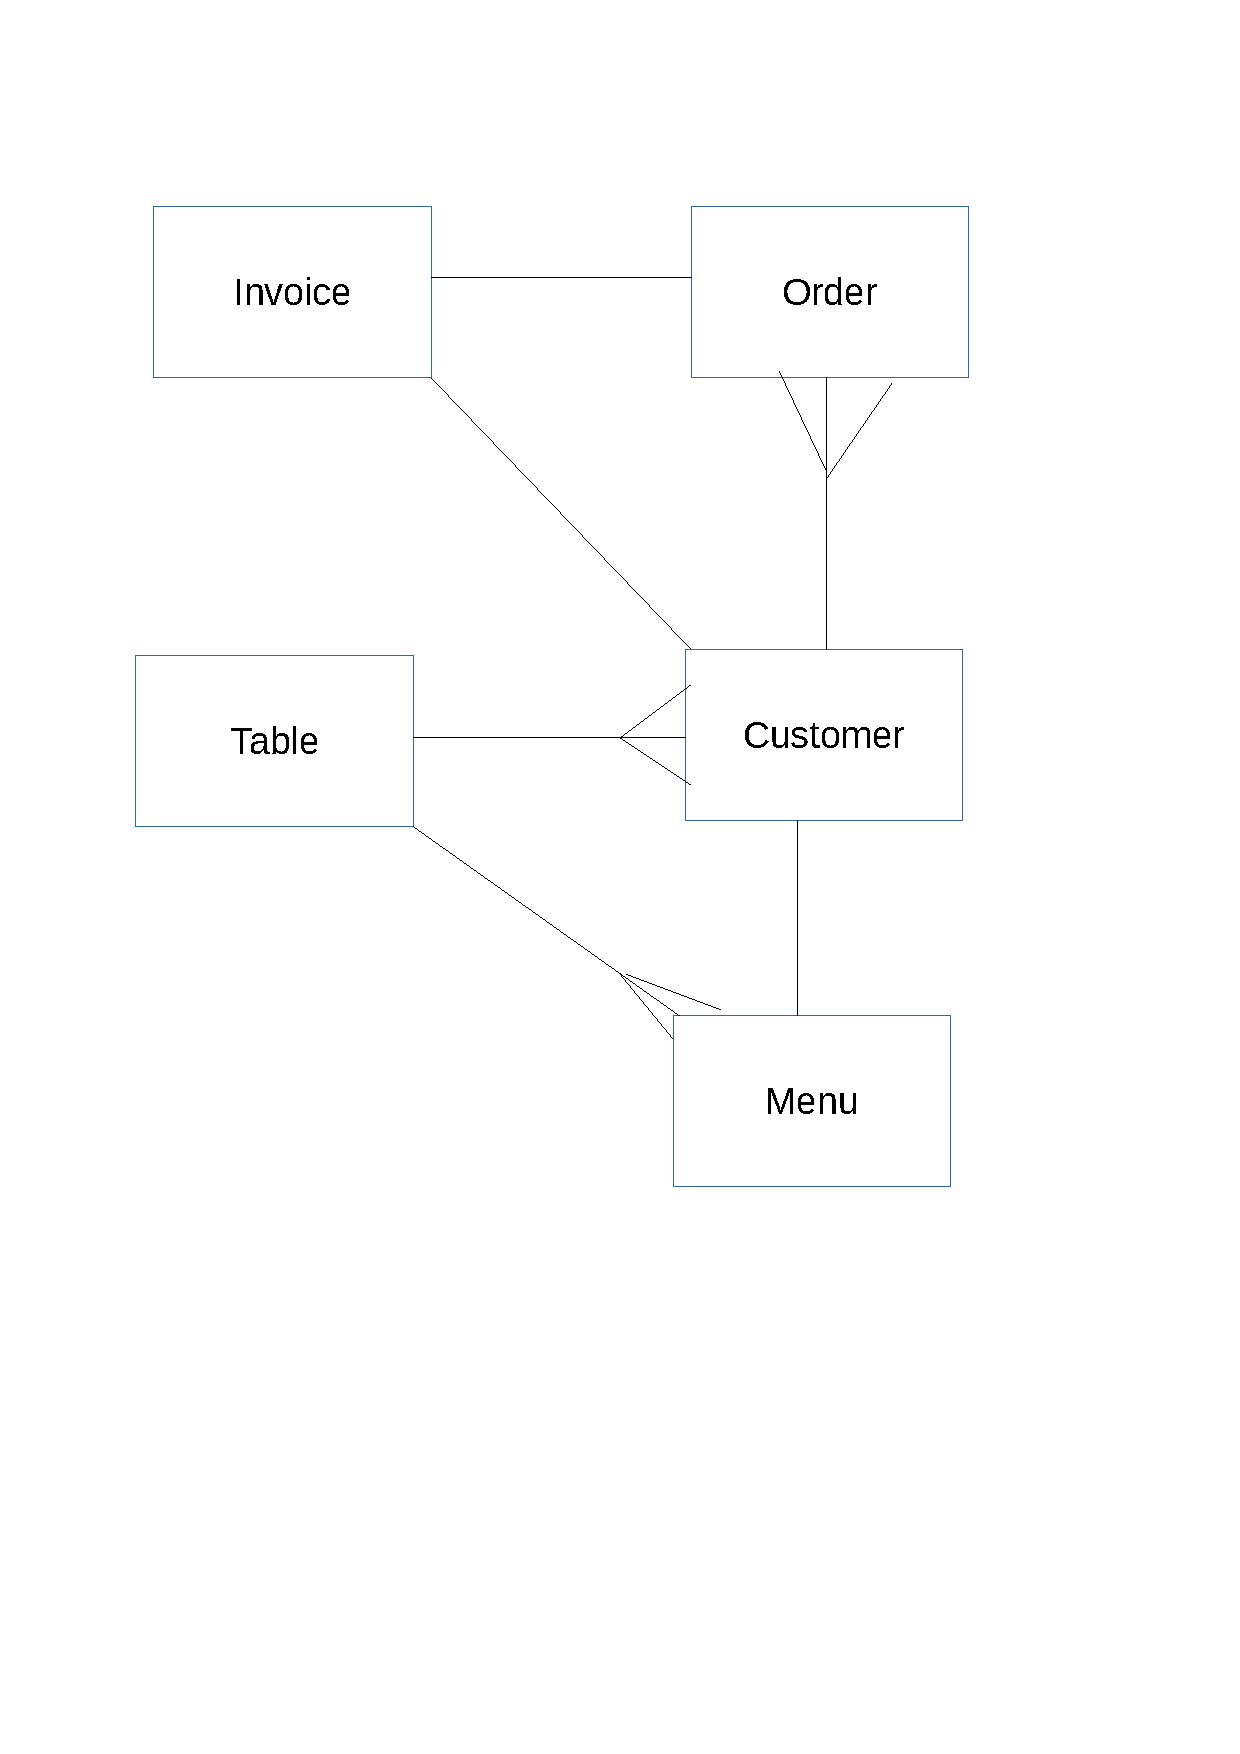
\includegraphics[height = 20cm]{./Design/Images/ERDiagram}
    \caption{Database ER Diagram} \label{fig:2ERDiagram}
\end{figure}
 

\subsubsection{Entity Descriptions}

Customer(\underline{CustomerID},\textit{BookingID}, \textit{OrderID},Date,Time,NoOfPpl,TableNumber) \\
Booking(\underline{BookingID},FirstName,LastName,TelephoneNo,BookingDate,BookingTime) \\
Menu(\underline{MenuID},\textit{Type}, MenuItem, ItemPrice) \\
ItemType(\underline{Type},TypeDescription) \\
Order(\underline{OrderID},TotalDrinkPrice,TotalDishPrice,TotalPrice) \\
OrderedItem(\underline{OrderItemID},\textit{OrderID},\textit{MenuID},Quantity) \\

\begin{center}
\textbf{Key} 
\\
*  Primary Key \\
- Foreign Key
\\
\end{center}


\begin{center}
\begin{tabular}{ | l |   }
    \hline
    \textbf{UNF} \\ \hline
	CustomerID \\
	Date \\
	Time \\
	NoOfPpl \\
	TableNumber \\
	MenuID \\
	MenuItem \\
	Type \\
	TypeDescription \\
	ItemPrice \\
	OrderID \\
	TotalDrinkPrice \\
	TotalDishPrice \\
	TotalPrice \\
	OrderItemID \\
	Quantity \\
	BookingID \\
	FirstName \\
	LastName \\
	TelephoneNo \\
	BookingDate \\
	BookingTime \\

     \hline
\end{tabular}
\label{tab:UnF}
\end{center}



\begin{center}
\textbf{1NF} \\
\begin{tabular}{ | l | l |   }
    \hline
    \textbf{Repeating} & \textbf{Non-Repeating} \\ \hline
	 *OrderID& *CustomerID\\
	*CustomerID & Date\\
	MenuID & Time\\	
	MenuItem & NoOfPpl\\
	Type & TableNumber\\
	 TypeDescription & BookingID\\
	ItemPrice &FirstName\\
	OrderItemID&LastName\\
	Quantity&TelephoneNo\\
	TotalDrinkPrice& BookingDate\\
	TotalDishPrice& BookingTime \\
	TotalPrice& \\
	
     \hline
\end{tabular}
\label{tab:1nF}
\end{center}

\begin{center}
\textbf{2NF} \\
\begin{tabular}{ | l | l |   }
    \hline
    \textbf{Repeating} & \textbf{Non-Repeating} \\ \hline
	 *OrderID& *CustomerID\\
	*CustomerID & Date\\
			 & Time \\	
	*OrderID & NoOfPpl\\
	TotalDrinkPrice & TableNumber\\
	TotalDishPrice & \\
	 TotalPrice &BookingID \\
	OrderItemID &FirstName\\
	Quantity&LastName\\
	          &TelephoneNo\\
	MenuID&BookingDate\\
	MenuItem&BookingTime \\
	Type& \\
	TypeDescription& \\
	ItemPrice& \\

     \hline
\end{tabular}
\label{tab:2nF}
\end{center}

\begin{center}
\textbf{3NF}
\end{center}

\begin{center}
\begin{tabular}{ | l |  }
    \hline
    \textbf{*CustomerID} \\ \hline
	-BookingID \\
	-OrderID \\
	Date \\
	Time \\
	NoOfPpl \\
	TableNumber \\

\hline
\end{tabular}
\label{tab:3nF}
\end{center}

\begin{center}
\begin{tabular}{ | l |   }
    \hline
    \textbf{*BookingID} \\ \hline

	FirstName\\
	LastName\\
	TelephoneNo \\
	BookingDate \\
	BookingTime \\
		
     \hline
\end{tabular}
\label{tab:3nF}
\end{center}


\begin{center}
\begin{tabular}{ | l |   }
    \hline
    \textbf{*MenuID} \\ \hline
	-Type\\
	MenuItem\\
	ItemPrice\\
	

     \hline
\end{tabular}
\label{tab:3nF}
\end{center}

\begin{center}
\begin{tabular}{ | l |   }
    \hline
    \textbf{*Type} \\ \hline

	TypeDescription\\
		
     \hline
\end{tabular}
\label{tab:3nF}
\end{center}

\begin{center}
\begin{tabular}{ | l |   }
    \hline
    \textbf{*OrderID} \\ \hline

	TotalDrinkPrice\\
	TotalDishPrice\\
	TotalPrice\\

     \hline
\end{tabular}
\label{tab:3nF}
\end{center}

\begin{center}
\begin{tabular}{ | l |   }
    \hline
    \textbf{*OrderItemID} \\ \hline

	-OrderID\\
	-MenuID\\
	Quantity \\
		
     \hline
\end{tabular}
\label{tab:3nF}
\end{center}



\subsection{SQL Queries} 
The following SQL Queries will be formated using Python.

\begin{sql}
   create table  Menu(
	MenuID integer,  
	MenuItem text,  
	ItemPrice real,  
	ItemTypeID integer, 
	primary key(MenuID)  
	foreign key(ItemTypeID) references ItemType(ItemTypeID))
\end{sql}
This creates a table called Menu with the attributes \textit{MenuItem}, \textit{ItemPrice}. The primary key is \textit{MenuID} and the foreign key is \textit{ItemTypeID} \\ \\

\begin{sql}
insert into OrderItem
where OrderID = ?, MenuID = ? and Quantity = ?

\end{sql}
This inserts a new OrderItem record with the attributes \textit{OrderID}, \textit{MenuID} and \textit{Quantity} \\ 

\begin{sql}
select *
from Booking
where BookingDate = TodaysDate
\end{sql}
This will return all of the records from the \textit{Booking} table that has the booking date matched with the present system date. The parameter TodaysDate holds the system date at that current time. \\ \\

\begin{sql}
delete from Booking
where BookingID = ?
\end{sql}
This will delete a booking from the \textit{Booking} table with the ID of \textit{BookingID} \\ \\

\begin{sql}
select *
from OrderedItems
where OrderID = ? 
\end{sql}
This will return all ordered items from an order.


\begin{sql}
update ItemPrice
from Menu
where MenuItem = ?
\end{sql}
This will update the price of an item from the menu with the item name of what the user chooses.

\section{Security and Integrity of the System and Data}

\subsection{Security and Integrity of Data}
To ensure that certain data is accurate such as prices of items, I will implememnt referential integrity to various tables in my database. Adding referential integrity would mean, if i perform a certain action to a record in a table which is also used in different table, the records in both tables will be both affected by this action. So if I updated a price of an item from the Menu table, this would also update the price of the item in a previous order.

This program will store personal information about customers such as the customer's name and telehphone number and so according to the data protection act, the information must not be kept longer than necessary. Information that is 2 years old will be deleted automatically, this will be done through the start up of the application. T he application will compare the records of the customers booking dates and the system dates, if there is a difference of 2 years, then the application will delete the records off the database. The information entered must also be accurate and so there will be many validations to make sure information is as accurate as possible.

\subsection{System Security}

I will implement a simple yet effective security feature where a password would need to be inputted by the user to access the program. The user would have to enter the correct password when accessing any data on the system, this will prevent unauthoried access to data. Unauthorised access is also supported by the Computer Misuse Act 1990 which covers: \\

\begin{itemize}
	\item unauthorised access to computer material
	\item unauthorised access to computer material with criminal intent
	\item unauthorised modification of computer material
\end{itemize}

\section{Validation}

\begin{center}
    \begin{tabular}{|p{2cm}|p{4cm}|p{2cm}|p{4cm}|}
        \hline
        \textbf{Item} & \textbf{Example} & \textbf{Validation / Verification applied} & \textbf{Comments}\\ \hline
      OrderedItem & Wonton soup &  Presence check Lookup check & To check that this item exists in menu database \\ \hline
	Telephone Number & 01325 419603 &Presence check Length check Number check & To make sure that a number has been entered which is 11 characters long \\ \hline
	FirstName & Rudolph & Presence check & To make sure that a name has been entered \\ \hline
	LastName & Moln & Presence check & To make sure that a name has been entered \\ \hline
	TableNumber & 4 &Look up check & Make sure that a non-existing number is not created \\ \hline
	MenuID & 63 & Lookup check & Make sure that a non-existing menuid is not created \\ \hline
	MenuItem & Crispy duck & Presence check Lookup check & Check that there aren't repeating menu items \\ \hline
	TotalPrice & 42.1 & Float check & Must be calculated from TotalDrinkPrice and TotalDishPrice \\ \hline
	Total Drink Price & 1.6 & Float check  Look up check& Must be calculated from the correct order and drink category \\ \hline
	Total Dish Price & 40.5 & Float check Look up check & Must be calculated from the correct order and dish category \\ \hline
	Number Of People & 9 & Range check & Must be a number but not an unrealistic number like 100 or 0 \\ \hline
	
    \end{tabular}
\end{center}

\section{Testing}

\begin{landscape}
\subsection{Outline Plan}

\begin{center}
    \begin{tabular}{|p{2cm}|p{5cm}|p{5cm}|p{4cm}|}
        \hline
        \textbf{Test Series} & \textbf{Purpose of Test Series} & \textbf{Testing Strategy} & \textbf{Strategy Rationale}\\ \hline
         1 & Test the flow of control between the user interfaces & Top-down testing &  \\ \hline
	2 & Test validation of data input is detected & Bottom-up testing & Each component will be tested once it is developed \\ \hline
	3 & Test information input is stored in the correct place & Black box testing & Each component will be tested once it is developed \\ \hline
	4 & Test algorithms to make sure that the output is correct & White box testing & Each component will be tested once it is developed \\ \hline
	5 & Test that the system fufils the specification & Acceptance testing & Each component will be tested once it is developed \\ \hline
	6 & Test database has referential integrity & Integration testing & Each component will be tested once it is developed \\ \hline
    \end{tabular}
\end{center}

\subsection{Detailed Plan}

\begin{center}
    \begin{longtable}{|p{1.5cm}|p{2.5cm}|p{2.5cm}|p{2cm}|p{2cm}|p{2cm}|p{2cm}|p{2cm}|}
        \hline
        \textbf{Test Series} & \textbf{Purpose of Test} & \textbf{Test Description} & \textbf{Test Data} & \textbf{Test Data Type (Normal/ Erroneous/ Boundary)} & \textbf{Expected Result} & \textbf{Actual Result} & \textbf{Evidence}\\ \hline
        1.01 & Test 'Change password' button functions correctly & Should direct user to change password interface  & Click Change password button & Normal & Change password interface should be displayed &  &  \\ \hline
        1.02 & Test Cancel button functions correctly on change password interface & Should redirect user to login screen  & Click Cancel button on change password interface & Normal & Change password interfact should close &  &  \\ \hline
        1.03 & Test interactive table functions correctly & Should direct user to the order details from the table selected  & Click on occupied table & Normal & Table  information screen should be displayed &  &  \\ \hline
        1.04 & Test unoccupied table functions correctly & Should direct user to 'add details to table'  interface  & Click on unoccupied table & Normal & 'Add details to table' interface should be displayed &  &  \\ \hline
        1.05 & Test Table information screen, add button functions correctly & Should direct user to add item  interface  & Click Add on table information screen & Normal & Add item interface should be displayed &  &  \\ \hline
        1.06 & Test table information screen, delete function correctly & Should change colour of delete button and red box will appear to indiciate deletion for items  & Click Delete button & Normal & Delete button should change colour and red boxes should appear next to each order item &  &  \\ \hline
        1.07 & Test 'Change password' button functions correctly & Should direct user to change password interface  & Click Change password button & Normal & Change password interface should be displayed &  &  \\ \hline
        1.08 & Test back arrow button functions correctly on table information screen & Should direct user to main screen & Click back arrow button & Normal & User redirected back to main screen should be displayed &  &  \\ \hline
        1.09 & Test 'Manage Bookings' button functions correctly on main screen & Should direct user to Manage Bookings interface  & Click Manage Bookings & Normal & Manage Bookings interface should be displayed &  &  \\ \hline
        1.10 & Test Add button functions correctly on Manage Bookings interface & Should direct user to create booking interface  & Click Add button & Normal & Create booking interface should be displayed &  &  \\ \hline
        1.11 & Test Cancel button functions correctly on create booking interface & Should redirect user to Manage Bookings interface  & Click Cancel button & Normal & User should be redirected to Manage Bookings interface &  &  \\ \hline
        1.12 & Test back arrow on manage bookings interface functions correctly & Should redirect user to main screen  & Click Change back arrow button & Normal & Main screen should be displayed &  &  \\ \hline
        1.13 & Test Delete button on Manage Bookings screen & Should direct user to bookings display interface  & Click Dlete button & Normal & Bookings display should be displayed  &  &  \\ \hline
        1.14 & Test back arrow button functions correctly on bookings display screen & Should redirect user to Manage Bookings interface  & Click back arrow button & Normal & User should be redirected to Manage Bookings interface &  &  \\ \hline
        2.01 & Verify password entered & The field cannot be left blank  & (Nothing), Treem & Erroneous, Normal & Error, Accepted &  &  \\ \hline
        2.02 & Verify new password entered at change password screen & The field cannot be left blank  & (Nothing), PineTree & Erroneous, Normal & Error, Accepted &  &  \\ \hline
        2.03 & Verify retype new password entered at change password screen & The field cannot be left blank  & (Nothing), PineTree & Erroneous, Normal & Error, Accepted &  &  \\ \hline
        2.04 & Verify old password entered at change password screen & The field cannot be left blank  & (Nothing) ,Treem & Erroneous, Normal & Error, Accepted &  &  \\ \hline
        2.05 & Verify Number of people entered at 'add details table' & The field cannot be left blank  & (Nothing),3 , pigs& Erroneous, Normal, Erroneous & Error, Accepted, Error &  &  \\ \hline
        2.06 & Verify MenuID entered at 'add item to order' interface & The field cannot be left blank  & (Nothing),3, 9552 & Erroneous, Normal, Erroneous & Error, Accepted, Error &  &  \\ \hline
        2.07 & Verify First Name entered at 'enter booking details' interface & The field cannot be left blank  & (Nothing), Milly, 63 & Erroneous, Normal, Erroneous & Error, Accepted, Error &  &  \\ \hline
        2.08 & Verify Last Name entered at 'enter booking details' interface & The field cannot be left blank  & (Nothing), Milk, 2 & Erroneous, Normal, Erroneous & Error, Accepted, Error &  &  \\ \hline
        2.09 & Verify Telephone Number entered at 'enter booking details'' interface & The field cannot be left blank  & (Nothing),01523 859372, 014829, 0158925 8295289 & Erroneous, Normal, Erroneous, Errorneous & Error, Accepted, Error, Error &  &  \\ \hline
        2.10 & Verify Table Number entered at 'enter booking details' interface & The field cannot be left blank  & (Nothing),7, Hey & Erroneous, Normal, Erroneous & Error, Accepted, Error &  &  \\ \hline
        2.11 & Verify Number Of People entered at 'enter booking details' interface & The field cannot be left blank  & (Nothing),3, Lisa & Erroneous, Normal, Erroneous & Error, Accepted, Error &  &  \\ \hline
        2.12 & Verify Date entered at 'enter booking details' interface & The field cannot be left blank  & (Nothing),06/05/13, Homer, 032/63/153 & Erroneous, Normal, Erroneous, Erroneous & Error, Accepted, Error, Error &  &  \\ \hline
        2.13 & Verify Time entered at 'enter booking details' interface & The field cannot be left blank  & (Nothing),18:12, Bart, 53:62 & Erroneous, Normal, Erroneous, Erroneous & Error, Accepted, Error, Error &  &  \\ \hline
        3.01 & Verify all table details entered are added to relevant database tables & Information should be added to the correct fields in customer, order and orderitem  tables. If necessary reservation table  & customer information, order information, orderitem information, if necessary reservation table & Normal &Added to customer, order and orderitem table. If necessary reservation table  & & \\ \hline
        3.02 & Verify that all details entered at 'enter booking details' interface are added to the reservation database & All of the information should be added to the correct field in the reservations table  & Reservation informationl & Normal & Added to the reservation table & &  \\ \hline
        4.01 & Verify password changed & Password should not successfully change if length is not bigger than 4 and old password does not match input old password   & -Try changing password with incorrect input and length of 2 new password, -Try changing password with new password having length of 2, - Try changing password with correct input and correct length&Error, Error, Accepted  & & \\ \hline
        4.02 & Verify add item function works correctly & Entering MenuID will return information based on that ID & Enter ID &  Normal & Return all information based on the ID  & & \\ \hline
        4.03 & Verify Total price calculation functions correctly & Adds up all items prices together to get a total & Enter items to order &  Normal & Calculates the total price based on items entered  & & \\ \hline
	4.04 & Check bookings displayed on correct day & Should display all bookings that match with system date & Create a range of bookings that have different dates & Normal& Displays correct bookings & & \\ \hline
         5.01 & Verify program fulfills the specification & Run through the program, testing all aspects to make sure the meet the objectives in the specification & Enter information in all places required input &  Normal & Program fulfils specification  & & \\ \hline
	6.01 & Verify menu item name updates in case an item is mistakenly spelt & Check  the item name is updated in all records that it appears in & Update name of a menu item (Wate to Water) & Normal & Wate should change to Water & & \\ \hline
	6.02 & Verify menu item price updates in case an item is mistakenly priced & Check the price of the item is updated in all records the item appears in & Update price of a menu item (0.060) to (0.60) & Normal & Price should change to 0.60 & & \\ \hline
	






    \end{longtable}
\end{center}
\end{landscape}
